% NWPU Bachelor LaTex Template

\documentclass{nwputhesis}


\usepackage{listings}
\usepackage{xcolor}
%\usepackage[space]{ctex}
%\usepackage{minted}
% link: <>
\lstset{
	basicstyle = \small	
}

\lstset{
	columns=fixed,       
	%numbers=left,   % 在左侧显示行号
	frame=none,     % 不显示背景边框
	backgroundcolor=\color[RGB]{245,245,244},   % 设定背景颜色
	keywordstyle=\color[RGB]{40,40,255},        % 设定关键字颜色
	numberstyle=\footnotesize\color{darkgray},  % 设定行号格式
	commentstyle=\it\color[RGB]{0,96,96},       % 设置代码注释的格式
	stringstyle=\rmfamily\slshape\color[RGB]{128,0,0}, % 设置字符串格式
	showstringspaces=false,                   % 不显示字符串中的空格
}


% Author Information
% Author Name
\nwpuAuthor{刘昭宏}
% Major
\nwpuMajor{飞行器控制与信息工程}
% Teacher Guide Name
\nwpuSupervisorFirst{布树辉}
% Time to Graduate
\nwpuGraduateTime{2022年6月}
% Title
\nwpuTitleFirstLine{集群无人机协同SLAM}

\pagestyle{plain}
\allowdisplaybreaks[4]

% document structure
\begin{document}

% define all eps,png,jpg,pdf files under figures/
\graphicspath{{figures/}}


%% cover and abstract


%%%%%%%%%%%%%%%%%%%%%%%%%%%%%%%%%%%%
% 封一
%%%%%%%%%%%%%%%%%%%%%%%%%%%%%%%%%%%%

\begin{titlepage}
\voffset 2.7cm
\begin{center}
\begin{center}
\begin{minipage}[c]{2.64cm}
\centering
\resizebox{!}{0.9cm}{%
\parbox{0.54cm}{\begin{tikzpicture}
  \draw[line width=0.1cm] (0,0) circle (2cm);
  \draw[line width=0.05cm] (0,0) circle (1.3cm);
  \fill[gray!15] (0,0) circle (1.3cm);
  \fill[white] (0,0) circle (0.9cm);
  \draw[line width=0.05cm] (0,0) circle (0.9cm);
  \fill[black] (-0.5,-0.73) .. controls (-0.35,-0.81) ..
	(-0.2,-0.8)  .. controls (0.15, -0.7) and (0.20,-0.60) .. 
	(0.35,-0.35)   .. controls (0.42, -0.24) and (0.6,-0.26) ..
	(0.6,-0.4)   .. controls (0.58,-0.50) and (0.49, -0.50) ..
	(0.45,-0.45) .. controls (0.4,-0.68) and (0.75, -0.7) ..
	(0.9,0) arc (360:250:0.9cm);
  \fill (-0.4,-0.4)--(-1.33,-0.4)--(1,1.1)--cycle;
  \fill (-0.37,-0.43)--(-0.2,-0.8)--(1.01,1.05)--cycle;
  
  \foreach \x/\txt in {0/N,1/O,2/R,3/T,4/H,5/W,6/E,7/S,8/T,9/E,10/R,11/N,12/~,13/P,14/O,15/L,16/Y,17/T,18/E,19/C,20/H,21/N,22/I,23/C,24/A,25/L,26/~,27/U,28/N,29/I,30/V,31/E,32/R,33/S,34/I,35/T,36/Y}
  {
    \node[scale=0.7,rotate=\x*-6.5-245] at (207+\x*-6.5:1.6cm) {\txt};
  };
  \foreach \x/\txt in {0/西,1/北,2/工,3/业,4/大,5/学}
  {
    \node[scale=1.25,rotate=\x*18-50] at (225+\x*18:1.65cm) {\CJKfamily{nwpu}\txt};
  };
  \foreach \x/\txt in {0/1,1/9,2/3,3/8}
  {
    \node[scale=1,rotate=\x*18-25] at (\x*18-115:1.1cm) {\bfseries\txt};
  };

\end{tikzpicture}
}
}
\end{minipage}
\hskip 0.8cm
\begin{minipage}[c]{8cm}
\fontsize{33}{33}\CJKfamily{nwpu} 西北工业大学
\end{minipage}
\end{center}
\vskip 0.7cm
\chuhao\CJKfamily{zhsong}{\bfseries 本科毕业设计(论文)}
\vskip 5cm

\sanhao\CJKfamily{zhhei} 题~~目 \hspace{0.2cm} \underline{\makebox[12.5cm]{\nwpuTitleFirstLineString}}

\vskip 2cm
{
\sihao\CJKfamily{zhsong} 专业名称  \underline{\makebox[7cm]{\nwpuMajorString}}
\vskip 0.7cm
\sihao\CJKfamily{zhsong} 学生姓名  \underline{\makebox[7cm]{\nwpuAuthorString}}
\vskip 0.7cm
\sihao\CJKfamily{zhsong} 指导教师  \underline{\makebox[7cm]{\nwpuSupervisorFirstString}}

\vskip 0.7cm

\sihao\CJKfamily{zhsong} 毕业时间  \underline{\makebox[7cm]{\nwpuGraduateTimeString}}
\vfill
}
\end{center}
\end{titlepage}

\CJKfamily{zhsong}\normalsize 
  %%封面页
\pagenumbering{Roman}

%%%%%%%%%%%%%%%%%%%%%%%%%%%%%%%%%%%%%%%%%%%%%%%%%%%%%%%%%%%%%%%%%%%%%%%%%
% 中文摘要
%%%%%%%%%%%%%%%%%%%%%%%%%%%%%%%%%%%%%%%%%%%%%%%%%%%%%%%%%%%%%%%%%%%%%%%%%

\renewcommand{\baselinestretch}{1.5}
\fontsize{12pt}{13pt} \selectfont

\chapter*{摘~~~~要}

\vspace{1em}

% 目的、方法、结果和结论称为摘要的四要素。

% 研究背景 1,2句话
无人机应用的场景越发广泛,机上搭载设备的多样化意味着其能实现更多的功能。
% 问题,一句话
但是,在GPS拒止环境下,无人机完成对自身周围的环境感知较为困难;单架无人机执行任务的效率和成功率也不能保证。
% 文章主旨
为了解决这一问题,本文主要研究集群无人机协同SLAM。SLAM技术使得无人机在GPS拒止环境下也能完成对环境的感知和对任务的决策,集群无人机则使得任务的完成更加高效。
% 试验方法及主要结论
本文通过对ROS、PX4的研究和SLAM理论知识及开源方案的学习,进行了两架配备有单目相机的无人机在gazebo仿真环境下进行视觉感知,完成定位与建图任务;这样协作的方案使得每一架无人机拥有自己的地图,并通过特定的融合策略得到一致估计的地图;最后,在真机上进行了视觉SLAM的实验,为进一步多机自主定位与建图创造了条件。
% 学术意义

\vspace{0.1in}
\noindent {\CJKfamily{zhhei} 关键词:} 无人机集群,协同SLAM



%%%%%%%%%%%%%%%%%%%%%%%%%%%%%%%%%%%%%%%%%%%%%%%%%%%%%%%%%%%%%%%%%%%%%%%%%
% 英文摘要
%%%%%%%%%%%%%%%%%%%%%%%%%%%%%%%%%%%%%%%%%%%%%%%%%%%%%%%%%%%%%%%%%%%%%%%%%


\chapter*{ABSTRACT}
\noindent 
\vspace{1em}

Drones are being used in a wider and wider range of scenarios, and the diversity of equipment on board means they can achieve more functions.
However, in the GPS denial environment, it is difficult for UAVs to sense their own surroundings; the efficiency and success rate of a single UAV mission cannot be guaranteed.
In order to solve this problem, this paper focuses on cluster UAV collaborative SLAM, which enables UAVs to sense the environment and make decisions about the mission even in GPS-denied environment, and cluster UAVs make the mission accomplishment more efficient.
In this paper, through the study of ROS, PX4 and theoretical knowledge of SLAM and open-source schemes, two UAVs equipped with monocular cameras perform visual perception and complete localization and map building tasks in a gazebo simulation environment; such a collaborative scheme allows each UAV to have its own map and get a consistently estimated map through a specific fusion strategy; finally, a real aircraft on Finally, experiments of visual SLAM were conducted on real aircraft, creating conditions for further multi-aircraft autonomous localization and map building.


\vspace{0.1in}
\noindent \textbf{Key Words:} SLAM,Multi UAVs
  %%摘要页


% content
\renewcommand{\baselinestretch}{1.25}
\fontsize{12pt}{12pt} \selectfont

\tableofcontents
\mainmatter


% main body
\renewcommand{\baselinestretch}{1.5}

\pagenumbering{arabic}
\setcounter{page}{4}

\renewcommand{\baselinestretch}{1.5}
\fontsize{12pt}{13pt}\selectfont

\chapter{绪论}\label{preface}

\section{研究背景}

当今阶段,无人机(Unmanned Aerial Vehicle)技术迅速发展,在单架无人机上配备的众多系统使单机已经能够执行各种各样的任务。
单架无人机已经可以在自然灾害的搜救、对高空电力线路的检查、日常交通及场所的安全巡查、农业播种等场景发挥出巨大的作用。
但是,单架无人机由于其运算资源有限、可搭载设备有限,在面对多种类的需求和复杂不可控的环境时,可能无法发挥出其作用;
%但是,面对复杂的应用环境和多样化的需求,单架无人机受自身软硬件条件的限制,仍然具有一些局限性;
%为了弥补单架无人机的局限性,由多架相同或不同型号的无人机组成多无人机系统,即无人机集群,协同定位,共同完成任务;
为了弥补单架无人机的局限性,可以使用集群无人机的方案,即由若干架相同型号或根据任务需求搭配不同型号的无人机组成一个多无人机系统,进行协同定位,并借此完成任务。

%通过集群的方式,能最大地发挥无人机的优势,又能避免由于单架无人机执行任务不佳或失败造成的不良后果,提高任务执行效率,扩展新的任务执行方式,从而达到提高系统可靠性,增强任务执行效果的目的。

集群是使无人机的优势较大化的一种手段,又可以达到有效降低单架无人机失误率和事故率,有效提升无人机在实际应用中的执行效率,大幅度拓展其任务执行方式,由此提升多无人机系统鲁棒性,有效提升任务完成率。对于无人机的自主导航,能够在进入未知的环境时掌握无人机的位置和姿态是使其成功的关键。尽管GPS对于掌握无人机的位置有巨大的u帮助,但仍存在普适性有限和准确度不高的问题;在一些特定场景下,比如室内狭小空间,对定位精度要求很高,GPS定位的局限性就被显露出来。而SLAM技术则可以仅通过自身携带的传感器,来完成这一任务,同时达到一定的精度;

SLAM技术,即同时完成定位与建图的任务,已有较为系统的理论和研究;SLAM于20世纪90年代左右由 Smith、Cheeseman 和Self提出。
%SLAM指的是机器人在未知环境中从一个未知位置开始移动,在移动过程中根据位置和地图进行自身定位,同时在自身定位的基础上建造增量式地图,实现机器人的自主定位和导航。由于其重要的理论与应用价值,被很多学者认为是实现真正全自主移动机器人的关键。
SLAM是指将机器人放置在陌生环境中,令其从未知位置开始运动,在行进中根据解算出的当前位置和初步构建的地图获取自身位置信息,基于此建立增量式地图,从而达成使机器人获得自主定位和导航能力的目标\cite{王晨捷2020无人机视觉}。



但是单平台SLAM受到传感器性能的限制,存在两点不足:一是测量距离受限,单平台常用的传感器如激光雷达,其最远有效距离为200米,不能够满足大场景定位建图的需要,任务效率比较低;二是单平台构建出的三维点云相对稀疏,不能表现出足够的场景信息\cite{高家隆2019多无人机协同定位与建图技术研究}。

因此集群无人机协同SLAM方案有望解决单机存在的制约问题,主要表现在两个方面:一是多机意味着多传感器,能在大范围场景进行同时定位与建图;二是多机协同SLAM可以通过建图覆盖的检测,构建更加稠密和精细的点云地图。

目前单机同时定位与建图已经相对成熟,但是多机SLAM由于其控制复杂、数据传输量大、信息处理速度受限、关键数据融合效率低等问题,仍然需要大量的理论研究和实验。

\section{研究内容及论文结构}
本文研究目标旨在实现一套能够在室内高精度环境或GPS拒止环境下使用视觉进行多机定位和大范围建图的多无人机协同SLAM的方案;其中:

\begin{enumerate}
	\item 在SLAM方面:掌握一些优秀的开源方案,选择各自优点做出一定的融合。并且有一套针对地图融合的方法。
	\item 在仿真方面:在ROS的gazebo仿真平台中实现一定的集群控制方法,能够控制多个无人机协同完成同时定位与建图的任务。
	\item 在真机方面:实现单机的视觉SLAM;在安全的前提下实现双机协同SLAM,将仿真环境下的协同SLAM算法在真机上完成验证,得到场景地图
\end{enumerate}

本研究内容是多机协作进行定位与建图,多机协同SLAM能大大提高任务进行的效率,但由于无人机数量多,协同上存在一定困难;研究内容分为三个模块:SLAM模块、仿真模块和真机模块。

SLAM模块的主要内容是实现一套可协作的SLAM方案,实现的步骤有:

\begin{enumerate}
	\item 研究传统的视觉SLAM的特征点提取、匹配、初始化、后端优化等技术,研究机器人的位姿估计技术;研究并了解SLAM技术的整体框架
	\item 研究CCM-SLAM方案,重点研究其协同的机制和方法,服务端到子端的信息传递和接口设计等
	\item 研究VINS-Fusion方案中的VIO方法,研究如何利用IMU与相机数据联合进行更加准确的位姿估计
\end{enumerate}

仿真模块的主要内容是在ROS的gazebo中研究如何实现多机协同的同时定位与建图,实现的步骤有:

\begin{enumerate}
	\item 首先研究PX4和MAVROS之间的通信方式,ROS的话题发布和订阅方式,研究如何用程序解锁一架无人机、使其进入Offboard模式、起飞悬停并降落
	\item 研究如何用程序发布话题,控制无人机按照航路点飞行
	\item 研究如何构建多机的仿真环境,如何对多机进行控制,其控制策略的选择,即集中式或分布式的多机编队控制
	\item 研究如何更改无人机的定位设置,将其从GPS定位改为视觉SLAM定位;并且完成单机的摄像头内容读取
	\item 研究如何在gazebo中载入其他场景,在场景中控制无人机飞行,并且对拍摄到的画面进行建图,完成自身定位
	\item 研究如何在gazebo中完成多机基于视觉的同时定位与建图,并且拼合地图,用第三方软件显示;研究多机的联合优化与协同方法
\end{enumerate}

真机模块的主要内容是控制无人机的协同飞行及通信,实现的步骤有:

\begin{enumerate}
	\item 研究无人机通过MAVROS,MAVLINK与地面站的通信方法,尤其是用于SLAM的关键数据的传输
	\item 研究多无人机与地面站之间的、多无人机之间的数据传输
	\item 研究多无人机之间的可变基线控制技术,如何设计一个详细的算法控制基线距离
\end{enumerate}

基于研究内容的层级关系,本论文的结构主要由四层构成,如图\ref{fig1}所示。
\vspace{10pt}
\begin{figure}[!ht]
\centering
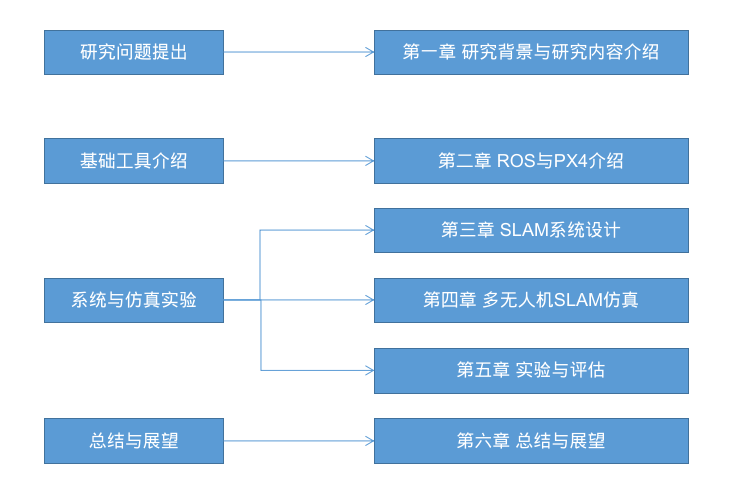
\includegraphics[width=0.8\textwidth]{structure.png}
\caption{论文结构 }
\label{fig1}
\end{figure}


第\ref{preface}章:主要介绍本文相关研究背景和现状;根据现阶段存在的问题,引出本文的研究方向和内容;从宏观的角度概括本文的内容,并且对问题做出概述。

第\ref{introduction}章:主要介绍研究中用到的ROS(Robotics Operating System,机器人操作系统)和PX4 AutoPilot飞控软件系统。

第\ref{System Overview}章:主要介绍SLAM的原理和作用,SLAM系统的基本流程,优秀的开源SLAM方案和地图融合的设计。

第\ref{Simulation}章:主要介绍仿真实验的情况,在ROS的gazebo环境中进行。

第\ref{experiment}章:主要介绍真机实验的情况,并且做出相应的评估。

第\ref{conclusion}章:总结本文研究中的创新点和有待改进之处,提出进一步研究的大致方向,展望未来的研究工作。



\chapter{ROS与PX4介绍}\label{introduction}

\section{ROS介绍}
本节主要对ROS平台进行介绍,包括ROS核心的消息机制和研究中要用到的gazebo仿真平台。

21世纪开始,随着人工智能研究的发展,催生出了一批智能机器人的研究项目;ROS诞生于2007年斯坦福大学AI实验室Morgan Quigley的STAIR(Standford Artificial Intelligence Robot)项目,其期望构建一个基于移动机器人+机械臂的原型;该项目于2008年受到Willow Garage公司关注,其决定用商业化手段来推进机器人的发展,使机器人平台能够更快地走进人们的日常生活;Willow Garage接手该项目后两年,2010年第一代ROS即ROS1.0发布;2013年,OSRF(Open Source Robotics Foundation)接管了ROS的维护工作和版本的升级工作,随后至2018年间,ROS的Indigo、Kinetic和Melodic版本相继发布。

ROS即Robotics Operating System,是一个针对机器人的开源、元级操作系统,在某些方面,ROS更像是一种机器人框架(robot framework);它提供类似于操作系统的服务,包含底层的驱动程序管理、底层的硬件描述,随后上升到软件程序之间的消息传递、功能包的管理和发布、也提供用于获得、编译、编写和多设备跨计算机运行代码所需的库等。换言之,ROS是由一套通信机制,开发工具,一系列应用功能和一个庞大的生态系统组成的集合,其目标为提高机器人研发中的软件复用率,不断完善他人的工作,进行更好的开发。

\subsection{ROS的消息机制} \label{2.1.1}

% ROS松耦合分布式通信+引出节点
ROS提供了一套松耦合分布式通信机制,这种分布式处理框架(又名Nodes),是以多个节点及节点之间的通信组成的。其中,节点(Node)和节点管理器(ROS Master)是ROS的核心概念,若干个节点在节点管理器下构建起来,共同实现特定的功能。

% 介绍节点的作用
每一个节点是一个独立的执行单元,由可执行文件构成,在程序中需要声明节点的名称;节点的名称必须唯一,否则ROS会舍弃掉时间节点靠前的节点;节点执行具体的任务进程,比如单目的ORB-SLAM2中,其节点为Mono,SLAM的任务仅靠一个节点完成。

% 介绍节点管理器
节点管理器是节点的控制中心,其作用是辅助节点的查找,帮助节点之间建立通信连接;还能提供节点的命名和注册等服务,以及提供了能够存储全局变量的配置的参数服务器。

\begin{figure}[!ht]
\centering
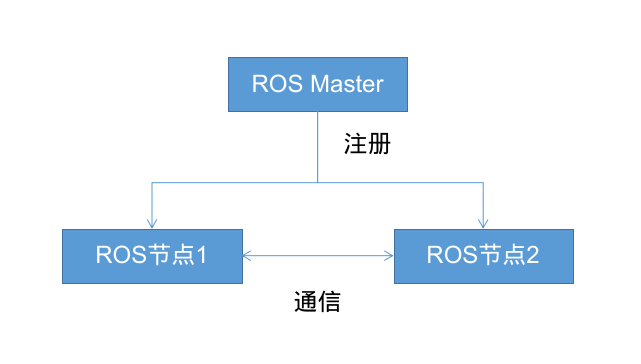
\includegraphics[width=0.6\textwidth]{ros_node.png}
\caption{ROS中的节点及通信} 
\label{fig2}
\end{figure}

% 介绍节点的通信
如图\ref{fig2}所示,节点在经过节点管理器注册后,可以建立节点之间的通信;常用的节点之间通信方式有两种,为话题(Topic)通信和服务(Service)通信:
\begin{enumerate}
	\item 话题通信是异步通信机制,数据为单向传输;数据的流向为发布者(Publisher)到订阅者(Subscriber);完成话题通信需要定义一个话题(Topic)及其消息(Message)的内容,之后通过发布者(Publisher)发布该话题,并且订阅者(Subscriber)订阅该话题的操作,完成数据的传输,消息的数据结构由.msg文件定义;话题通信可以完成多对多的信息传递。
	\item 
	服务的通信机制则为同步,数据为双向传输;数据的流向为客户端(Client)与服务器(Server)之间的交互;完成服务的通信需要客户端向服务器发送请求,服务器完成任务处理后,向客户端返回应答数据,表示请求和应答的数据结构定义在.srv文件中;服务通信一般用于逻辑判断,比如询问一项任务是否执行完毕,是一对多的节点处理关系。
\end{enumerate}

% 介绍Topic的编程
发布和订阅话题的方法,发布者和订阅者类似,以发布者为例:先实例化一个发布者对象,定义发布的话题名称、数据类型和队列长度,最后对消息进行定义并发送,简单的逻辑代码如下:
\begin{lstlisting}[language={C++}]
ros::NodeHandle n;  // define ros node handle
// define a publisher
ros::Publisher pub = n.advertise<'message type'>
	("topic name", `queue length`);
// publish message
pub.publish(message);
\end{lstlisting}

需要注意的是,订阅者则需要声明并定义一个回调函数,在实例化Subscriber的对象后,通过ROS的spin()函数,循环等待回调函数获得话题消息。

% 介绍Service的编程
客户端-服务器模型下的服务通信,则比话题的发布和订阅复杂;客户端的编程实现中,需要设置阻塞函数,其作用是直到发现对应的服务时才向下进行,否则程序被截止在该位置;如果对应的服务被发现,阻塞函数通过,之后创建客户端并且进行数据的设置,完成服务调用的请求,其代码实现如下:
\begin{lstlisting}[language={C++}]
// wait for right service
ros::service::waitForService("service name");
// create a client, connecting to service
ros::ServiceClient client = n.serviceClient
	<'data type'>("service name");
// call service
client.call(srv);
\end{lstlisting}

服务器的实现与订阅者类似,需要一个回调函数,如果收到了客户端发来的请求,则会触发回调函数,程序向下进行,否则将循环等待回调函数收到客户端发来的请求。

% 介绍参数服务器
除此之外,ROS中还有参数(Parameter)或参数服务器的概念,其作用类似全局共享字典,节点可以进行访问,适合存储一些和系统配置相关的静态非二进制的参数,以供节点读取。


\subsection{gazebo仿真} \label{2.1.2}
% 简单介绍gazebo及其功能
gazebo是ROS自带的仿真软件,其功能有构建具有运动属性的机器人仿真模型,提供了一些针对CAD和soildworks等2D、3D设计软件的接口;gazebo还具有构建现实世界的各种场景的仿真模型的功能,能够在gazebo环境中建立一个与现实十分相似的场景用于算法验证;在传感器的仿真上,gazebo拥有一个强大的传感器模型库,比如单目相机、双目相机、深度相机等,还可以根据需求自行配置传感器的类型,实现多传感器融合;除此之外,gazebo还引入了现实世界的物理性质,如重力的影响,使仿真环境更加贴近现实。

gazebo的仿真环境中,其文件大致可以分为三种类型:model,world,launch文件;同时,这三种文件也代表了不同的分级;

\begin{figure}[!ht]
	\centering
	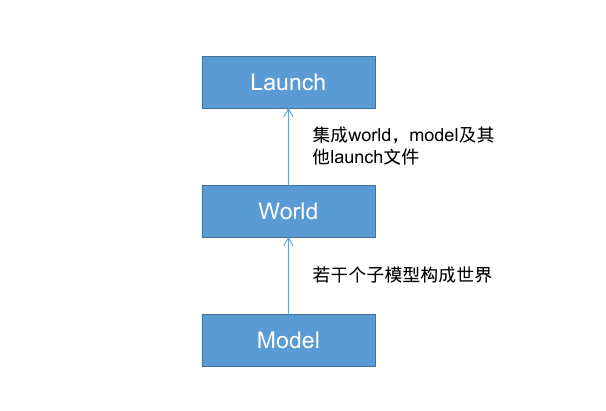
\includegraphics[width=0.6\textwidth]{gazebo.png}
	\caption{model,world,launch层级关系} 
	\label{fig3}
\end{figure}

如图\ref{fig3}所示:
\begin{enumerate}
	\item model(模型)是gazebo环境中的元级元素,也就是最底层文件,比如环境中的树木、双目相机、无人机、墙壁、桌子等都是model级别的物体。model由sdf文件和config文件构成;sdf文件用HTML或XML标签语言描述了该模型的主要内容,包括模型的构建方法、模型中对其他模型的调用以及连接方式、模型的位姿等参数配置;而config文件中记录了模型的作者及联系方式、模型的版本、模型的命名和描述等信息。由于模型具有可拼接的属性,因此一个模型可以由若干个模型组成。
	\item
	world(世界)文件将模型集成起来,包含模型和物理性质的设置,是gazebo环境中的中层文件。该层与model层相同,都无法完成代码对模型的直接控制。
	\item 
	launch文件是集成了model,world以及其他launch文件的gazebo中最顶层的文件;launch文件不同于model和world文件,其可以通过代码完成对模型的直接控制;launch文件在ROS中拥有定义,其以XML标签语言书写,可以在launch文件中完成嵌套其他launch文件、命名重映射、设置参数、启动ROS节点等任务;在ROS中有与launch文件对应的指令roslaunch,用于启动该launch文件。
\end{enumerate}

% 是否还需要一些别的内容

\section{PX4 AutoPilot}
% 本部分介绍PX4
PX4是一款专业级开源飞控,也可以称之为自动驾驶仪;因其应用的平台不局限于飞行器,在竞速和物流应用的地面车辆和潜水艇等载具上也可以用其进行控制。PX4由来自学术界和业界的顶级开发商开发,并且配套有活跃的全球论坛社区,其software的源码在github上保持着issue和pull request的更新,是应用十分广泛的一款飞控软件。需要注意,PX4 Software和Pixhawk4并不是同一概念,前者为飞控软件,而后者为飞控硬件。PX4软件的内部包含了针对不同机型(包括多旋翼、固定翼和VTOL垂直起降固定翼等)的控制律设计,还包含了强大的飞行模式设计和安全设计。PX4还可以作为核心应用在更广阔的平台,比如使用了QGroundControl地面站、Pixhawk硬件、基于计算机、相机等的使用MAVLink协议的MAVSDK融合等。


\subsection{FailSafe机制} \label{2.2.1}
% 简单介绍FailSafe
FailSafe机制,即安全生效机制,其含义为:当错误发生时,对飞机进行保护或恢复到安全的状态,避免错误可能导致的不良后果。PX4的FailSafe系统是可编辑的,意味着开发者可以根据自身的需求设置对FailSafe的触发,以保证在安全的情况下实验或完成任务。FailSafe系统被触发后,一般有自动着陆、保持位置或返回特定的航路点几种反馈措施。

安全生效机制监控的主要情况有:
\begin{enumerate}
	\item 低电量;该情况在仿真中影响较小,但在真机实验中,低电量可能意味着无法安全返航,因此必须由安全生效机制介入;
	\item 远程控制信号丢失,如遥控器信号丢失;
	\item 位置信息丢失,比如GPS信号弱,对位置的估计不够精确,可能会影响任务的完成情况,因此由安全生效机制介入;
	\item 场外连接丢失;是指进入到Offboard模式后,丢失了与计算机之间的连接,导致计算机无法通过Offboard程序对无人机进行控制;
	\item 数据链丢失;一般是指丢失了与GCS(Ground Control Station,地面站)之间的数传连接;
	\item 超出地理围栏;Geofence即地理围栏,是执行任务前设置的无人机可活动区域,高度一般不设限;
	\item 任务判断;防止在新的起飞位置上执行先前的任务;
\end{enumerate}

% bug实例
PX4版本更新后,如果直接输入commander takeoff指令,可能会遇到无法起飞的情况;同时在PX4终端中,会提示FailSafe activated,即安全生效模式被激活;一般遇到这种情况,需要在PX4终端的字里行间和地面站QGC的信息提示中去分析问题原因。比如在仿真中遇到No RC的情况,RC即Remote Control,对于SITL(软件在环仿真)是没有遥控器的信号输入的,因此需要在QGC中打开virtual joystick (虚拟摇杆),否则FailSafe模式会由于没有RC保持给飞机上锁。

\subsection{EKF与飞行模式} \label{2.2.2}

% 什么是ECL EKF
一般ECL与EKF会同时出现,ECL即Estimation and Control Library,状态估计和控制库;EKF即Extended Kalman Filter,扩展卡尔曼滤波,是一种优化算法。两者的结合是使用扩展卡尔曼滤波方法的状态估计与控制库,其作用是加工传感器的数据,并对IMU(惯性测量单元)加工的速度和位置、四元数表示的旋转矩阵、风速和磁罗盘得到的方向等信息进行加工处理和估计。EKF使用IMU、磁力计、高度计、GPS、测速仪等传感器。

为了将传统的气压计+GPS的高度与位置估计更改为使用视觉信息的高度与位置估计,需要修改EKF传感器的相关参数,这里指用于多旋翼和固定翼的基于扩展卡尔曼滤波的高度和位置估计。

\begin{enumerate}
	\item 
	\textit{EKF2\_AID\_MASK} (Integer bitmask controlling data fusion and aiding methods),该参数决定了GPS数据的融合方法;默认设置的参数为0,其意为使用GPS数据作为定位;如果修改为视觉定位(vision position fusion),需要将该参数改为3。
	\item 
	\textit{EKF2\_HGT\_MODE} (Determines the primary source of height data used by the EKF),该参数决定了EKF首选的高度信息传感器;默认参数设置为0,使用气压器得到高度;如果修改为视觉定位,则需要将该参数改为3。
\end{enumerate}

在启动仿真之前,需要根据信息融合的类型更改以上两个参数,修改参数的方式有以下两种:
\begin{enumerate}
	\item 更改rcS文件中的参数配置;rcS文件属于脚本文件,用于配置系统,PX4需要修改的rcS文件位于\textit{ROMFS/px4fmu\_common/init.d-posix/rcS}中,rcS文件中的参数被修改后,需要删除ROS的eeprom中存储的参数文件(该文件用于快速预加载参数);但该方法存在一些问题,需要在launch中特殊指明PX4使用的rcS文件地址,否则PX4会从默认的build文件夹中选择rcS文件进行参数配置。
	\item 
	更改地面站中的参数配置;使用QGC地面站,直接在参数设置中更改位置和高度估计的传感器,这种方式免去了每次更改参数后需要删除ROS参数缓存文件的麻烦。
\end{enumerate}

飞行模式决定了飞行器对RC远程控制输入的回应,以及在全自主的飞行过程中飞行器如何控制自身的运动;飞行模式为操作者主要提供了不同种类和程度的自动控制协助,飞行欧式的切换可以由遥控器和地面站完成。下面介绍几种主要的飞行模式(对于多旋翼无人机):
\begin{enumerate}
	\item 
	Manual/Stabilized Mode,手动/增稳飞行模式;是最常用的飞行模式,手动模式即操纵手通过手中的遥控器(RC)控制飞机的滚转、俯仰、油门和前后左右的移动;增稳模式也是由操纵手操纵,但引入了内部控制律,使得遥控器输入到飞机运动的表现更加平滑、易控,这是由其内部的控制律决定的;一般情况下为了防止飞机过于剧烈的运动,都采用增稳模式进行飞行。
	\item 
	Position Mode,定点模式;其主要特点是当操纵杆释放或回归中心时,飞机会保持在3D空间中的一个定点位置处,并且自动解算出相应的力去补偿风和其他的干扰力。该模式是对于新手最安全的模式。
	\item
	Altitude Mode,定高模式;其主要特点是当操纵杆释放或回归中心时,飞机会保持固定高度,但不会去平衡风等其他干扰所造成的水平位置的漂移。
	\item 
	Offboard Mode,场外模式;指通过电脑连接或地面站连接,使飞机按照设定的位置、速度或高度等参数飞行,该模式通过MAVLink与场外设备传递信息,是仿真中使用的主要模式。
	\item 
	其他模式,如圆轨迹模式、起飞降落模式、跟随模式、返回模式等。
\end{enumerate}

\subsection{联合MAVROS的Offboard模式} \label{2.2.3}
本小节主要介绍在Offboard模式下,使用ROS节点通过MAVROS向PX4发送信息,使无人机起飞降落、按航路点移动等。

Offboard模式下的无人机正常起飞,需要首先解锁,然后切换飞行模式(默认手动模式)到Offboard模式,但是需要在切换模式前,以不低于2$Hz$的频率发布一些设定点(setpoints),具体实现起飞的步骤如下:

\begin{enumerate}
	\item 
	连接fcu(MAVROS),判断的标准是MAVROS消息类中的state是否表示为连接;如果连接上则可以继续执行,未连接上则通过spin()函数循环等待。
	\item 
	设定setpoints的坐标值,并以不低于2$Hz$的频率发送一些点。
	\item 
	解锁,解锁成功后切换到Ofboard模式并起飞。
\end{enumerate}

其程序的实现如下:

首先是需要的头文件定义,其包括了C++的基本库,MAVROS的消息相关库,和ROS库;
\begin{lstlisting}[language={C++}]
//
// Created by hazyparker on 2022/1/11.
// realize mode switching and anto takeoff and landing

#include <iostream>
#include <ros/ros.h>
#include <geometry_msgs/PoseStamped.h>
#include <mavros_msgs/SetMode.h>
#include <mavros_msgs/State.h>
#include <mavros_msgs/PositionTarget.h>
\end{lstlisting}

之后需要在main函数之前,声明定义回调函数,其中包括对当前状态和当前位置的回调函数和消息定义:
\begin{lstlisting}[language={C++}]
// record current state
mavros_msgs::State current_state; /* NOLINT */

// callback function for Subscriber stats_sub
void state_cb(const mavros_msgs::State::ConstPtr& msg){
current_state = *msg;
}

// record current pose
geometry_msgs::PoseStamped current_pose; /* NOLINT */

// callback function for Subscriber for local_pos_sub
void local_cb(const geometry_msgs::PoseStamped::ConstPtr& msg){
current_pose = *msg;
}
\end{lstlisting}

在main函数中,首先要定义ROS节点和句柄,实例化飞行模式和当前位置信息的订阅者和发布者,然后以一定的频率发送一些点,以便切换到Offboard模式:
\begin{lstlisting}[language={C++}]
// init ros node
ros::init(argc, argv, "offb_node");

// create node handle
ros::NodeHandle nh;

// define subscribers and clients
ros::Subscriber state_sub = nh.subscribe<mavros_msgs::State>
("mavros/state", 10, state_cb);
ros::Subscriber local_pos_sub = nh.subscribe<geometry_msgs::PoseStamped>
("mavros/local_position/pose",10,local_cb);
ros::Publisher local_pos_pub = nh.advertise<geometry_msgs::PoseStamped>
("mavros/setpoint_position/local", 10);
ros::ServiceClient arming_client = nh.serviceClient<mavros_msgs::CommandBool>
("mavros/cmd/arming");
ros::ServiceClient set_mode_client = nh.serviceClient<mavros_msgs::SetMode>
("mavros/set_mode");

//the set-point publishing rate MUST be faster than 2Hz
ros::Rate rate(20.0);

// wait for FCU connection
while(ros::ok() && !current_state.connected){
ros::spinOnce();
rate.sleep();
ROS_INFO("wait for fcu connecting...");
}
ROS_INFO("fcu connected successfully");

// set pose
geometry_msgs::PoseStamped pose;
pose.pose.position.x = 0;
pose.pose.position.y = 0;
pose.pose.position.z = 2;

//send a few set-points before starting
for(int i = 100; ros::ok() && i > 0; --i){
local_pos_pub.publish(pose);
ros::spinOnce();
rate.sleep();
}
\end{lstlisting}

最后首先发送指令,使无人机解锁,之后使其切换到Offboard模式,完成起飞并到达目标点的指令:
\begin{lstlisting}[language={C++}]
int main(int argc, char **argv){


mavros_msgs::SetMode offb_set_mode;
offb_set_mode.request.custom_mode = "OFFBOARD";

mavros_msgs::CommandBool arm_cmd;
arm_cmd.request.value = true;

ros::Time last_request = ros::Time::now();
ROS_INFO("Off boarding");
while(ros::ok()){
if( current_state.mode != "OFFBOARD" &&
(ros::Time::now() - last_request > ros::Duration(5.0))){
if( set_mode_client.call(offb_set_mode) &&
offb_set_mode.response.mode_sent){
ROS_INFO("Off-board mode enabling...");
}
last_request = ros::Time::now();

} else {
if( !current_state.armed &&
(ros::Time::now() - last_request > ros::Duration(5.0))){
if (current_state.mode != "OFFBOARD") ROS_INFO("Off board mode was shut unexpectedly");
if( arming_client.call(arm_cmd) &&
arm_cmd.response.success){
ROS_INFO("Vehicle armed");
}
last_request = ros::Time::now();
}
}

local_pos_pub.publish(pose);

// wait until reach set point
ros::spinOnce();
// define Point: current position and set point position (expected)
geometry_msgs::Point curr,aim;
curr = current_pose.pose.position;
aim = pose.pose.position;
double dist = sqrt(pow((curr.x - aim.x), 2) +
pow((curr.y - aim.y), 2) + pow((curr.z - aim.z), 2));
if(dist < 0.1){
ROS_INFO("reached the goal...");
break;
}
rate.sleep();
}

}

return 0;
}
\end{lstlisting}












\renewcommand{\baselinestretch}{1.5}
\fontsize{12pt}{13pt}\selectfont

\chapter{SLAM系统设计} \label{System Overview}
本章节主要介绍SLAM的概念和原理、一个基本SLAM系统的框架、两个优秀的开源SLAM框架和地图融合算法。

\section{SLAM系统}
同时定位与建图(SLAM,simultaneous localization and mapping)技术,其希望是机器人在对环境和自身所处在环境中的位置未知的情况下,在反复的运动过程中不断观测到的地图特征完成自身位置的定位和姿态的确定,之后再根据自身位置对环境构建增量式的地图,从而达到同时定位与建图的目的。


\subsection{成像原理及相机参数} \label{3.1.2}
在各种SLAM中,视觉SLAM由于其传感器(光学相机)造价较低的原因,成为了SLAM中最常用的方式,要了解使用相机的视觉SLAM的原理,首先需要了解相机的成像原理及其参数。

如图\ref{fig4},可以用小孔成像的原理简单地解释针孔相机的模型:
\begin{figure}[!ht]
	\centering
	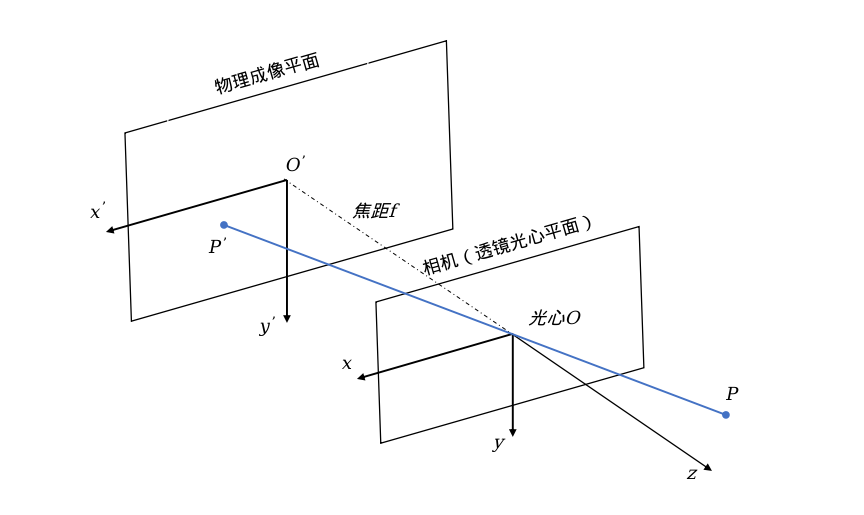
\includegraphics[width=0.6\textwidth]{camera.png}
	\caption{针孔相机模型} 
	\label{fig4}
\end{figure}

$Oxy$平面为相机光心(垂直主光轴)所在的平面,称其为相机平面,对应的$O-x-y-z$坐标系即为相机坐标系;$O'x'y'$平面为物理成像平面,$\bar{OO'}$的长度为焦距$f$;在现实世界中有一点$P$,设其在相机坐标系下的坐标为$[X, Y, Z]^T$,其经过小孔$O$投影后,在相机坐标系下落在像素平面上的坐标为$[X', Y', Z']^T$。

理论下,小孔成像为倒立的实像,但在实际的相机中,成像被人为旋转,成正立的像,因此不考虑坐标系正负号的影响,由相似三角形关系,有:

\begin{equation}
\frac{Z}{f}=\frac{X}{X'}=\frac{Y}{Y'}
\end{equation}


在此基础上,定义像素坐标系。像素坐标系为二维坐标系,在物理成像平面上;像素坐标系的原点位于图像的左上角,横轴为$u$轴,向右与$x$轴平行,纵轴为$v$轴,向下与$y$轴平行,则可以得到像素坐标与$P'$坐标的关系为:

\begin{equation}
\begin{cases}
u=\alpha X'+c_x=\alpha f \cfrac{X}{Z}+c_x \\
v=\beta Y' +c_y=\beta f  \cfrac{Y}{Z}+c_y \\
\end{cases}
\end{equation}


其中,$\alpha$和$\beta$为横轴和纵轴的缩放倍数,$c_x$为图像横向像素的一半,$c_y$为图像纵向像素的一半。令$f_x=\alpha f$,$f_y=\beta f$,将像素坐标系下的坐标转换为齐次坐标:

\begin{equation}
\begin{bmatrix}
u\\v\\1
\end{bmatrix}=
\frac{1}{Z}
\begin{bmatrix}
f_x & 0 & c_x\\
0   & f_y & c_y\\
0 & 0 & 1
\end{bmatrix}
\begin{bmatrix}
X\\Y\\Z
\end{bmatrix}=
\frac{1}{Z} \bf{KP}
\end{equation}


则得到了相机的内参矩阵(Camera Intrinsics)$\bf{K}$。通常情况下,对于焦距固定的相机(或定焦镜头),其出厂之后内参矩阵是固定的;如果无法从厂家得到相机的内参,可以使用标定的方法获得相机的内参矩阵,常见的标定算法有张正友标定法\cite{Gao2017SLAM}。

除相机的内参外,还有相机外参(Camera Extrinsics)的定义;相机的外参由其旋转矩阵$\bf{R}$和平移向量$\bf{t}$构成。对于$P$点而言,其在相机坐标系(像素坐标平面)下的坐标应为其在世界坐标系下的坐标根据相机相对于世界坐标系的位姿所变换得到的,相机的位姿即由其外参决定,则世界坐标系下$P$点的坐标$\bf{P_w}$在相机坐标系下的坐标为:


\begin{equation}
Z
\begin{bmatrix}
u\\v\\1
\end{bmatrix}=
\bf{K(RP_w+t)}
\end{equation}

\subsection{视觉SLAM的基本步骤} \label{3.1.3}

经典的视觉SLAM框架如图\ref{fig5}所示:

\begin{figure}[!ht]
	\centering
	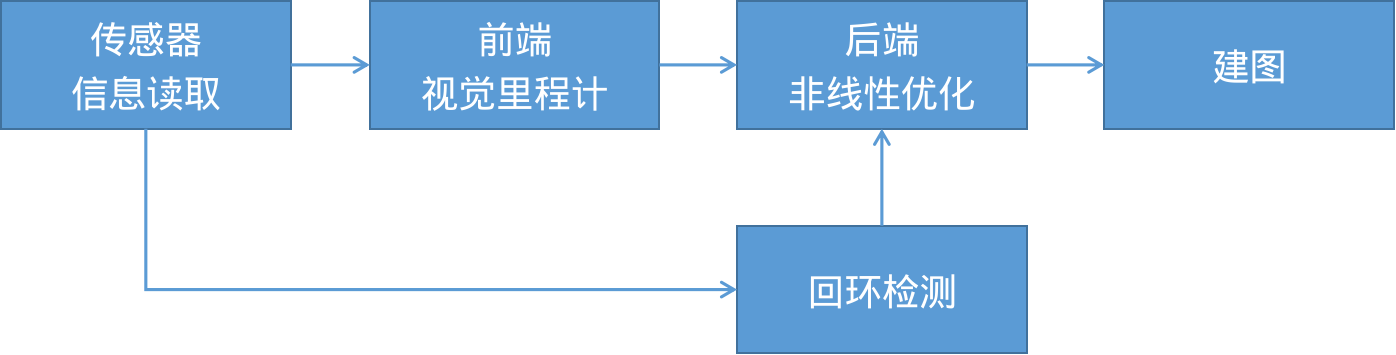
\includegraphics[width=0.7\textwidth]{SLAM.png}
	\caption{经典视觉SLAM框架} 
	\label{fig5}
\end{figure}

经典视觉SLAM流程包括以下基本步骤:
\begin{enumerate}
	\item 
	传感器信息读取。主要为相机图像的读取以及一些预处理步骤,在不同的视觉SLAM算法中,可能还涉及惯性测量元件信息的读取和预处理。
	\item 
	前端视觉里程计(Visual Odometry)。视觉里程计的功能是从相邻的几帧图像之中,根据几何约束,得到相机的运动;并且通过记录地图点(路标)与相机的相对位置,构建局部地图。
	\item 
	后端(非线性)优化(Optimization)。后端主要涉及滤波与非线性优化算法,其目的是减少传感器的误差,完成对运动的相机和周围环境的不确定性的估计。
	\item 
	回环检测(Loop Closure Detection)。回环检测的作用是使机器人能够分辨出当前面临的场景是否曾经来到过,解决位置估计的误差随时间累计,发生漂移的问题;并且消除累计误差,最终得到全局一致的轨迹和地图。
	\item 
	建图(Mapping)。建图即根据前端里程计和后端优化得到的地图点(路标点),构建地图。
\end{enumerate}

% 视觉里程计
视觉里程计是SLAM的关键,其基本完成了同时定位与建图的任务。视觉里程计的实现主要有两种方法:特征点法和直接法。

% 特征点法
特征点法作为很长时间以来视觉里程计的主要方法,其特点是比较稳定,在光照差异大和画面中有动态物体的情况下也能较好地完成任务。特征点法的核心在特征点的提取与匹配;提取即从每帧图像中找到可以代表图像特征的点,辨识度更高的点。

\begin{figure}[!ht]
	\centering
	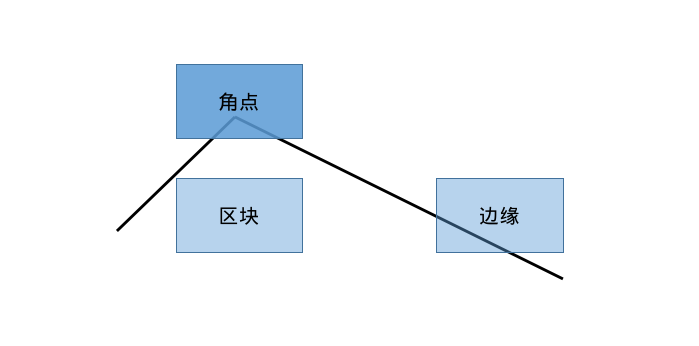
\includegraphics[width=0.6\textwidth]{corner.png}
	\caption{角点、边缘、区块} 
	\label{fig6}
\end{figure}

特征点的一种方法是使用角点。如图\ref{fig6},可以把一张图像中的内容分为角点、边缘、区块三种类型。可以发现,指出某两张图像中出现的统一区块是最难以实现的,因为存在大面积相同的色块,无法确定具体点的匹配;其次是边缘,其具有一定的特征,但沿边缘行进,仍可能出现相同的局部特征,造成误匹配;因此选择其中最具有特征角点作为特征。性能较好、比较稳定的角点有SIFT、SURF,ORB等。

% 对极几何与三角测量
在完成特征点提取与匹配后,根据不同的传感器类型,有不同的得到相机位姿的方法。对于传统的单目相机传感器,可以使用对极几何约束,得到相机的运动,并通过三角测量的方法恢复地图点相对于每时刻相机的位置。

% 直接法
前端视觉里程计的另一种方法是直接法,由光流法演变而来。光流法与特征点法不同,特征点法使用特征点的描述子来完成特征匹配,而光流法可以跟踪特征点的运动,这样就无需进行大量的描述子匹配运算。直接法可以弥补特征点法的一些缺陷。


% 优化
后端优化主要有两种方法,滤波和非线性优化。拓展卡尔曼滤波EKF及其演变出的粒子滤波方法等,在早期的SLAM设计中应用十分广泛。但随着非线性优化方法的普及,现在的SLAM方案多用BA图优化及位姿图优化的方法,并且有可以使用的ceres和g2o库。

% 回环检测
回环检测在判断场景是否曾经来过时,一般用的是词袋模型(Bag of Words)\cite{zhang2010understanding},根据图像中是否存在同样的几种相似特征来判断是否在外观上相似。

% 建图
建图根据地图的需求,可以分为用于定位的稀疏地图,用于导航、重建的稠密地图和用于交互的语义地图。按照地图的分类,可以分为拓扑地图和度量地图两种;拓扑地图着重与图节点之间的连通性,而度量地图则能够精确地表示出地图点相对于相机的位置。


\subsection{对极几何约束与三角测量} \label{3.1.4}


\section{ORB-SLAM2}

ORB-SLAM2是由萨拉戈萨大学的Raúl Mur-Artal开发,可以用在单目、双目、RGB-D深度相机的视觉SLAM系统。

\subsection{ORB特征点及描述子} \label{3.2.1}

% 简单介绍 
ORB特征点是上文\ref{3.1.3}提到过的特征点的一种,它的全称是Oriented FAST and Rotated BRIEF;其中,FAST是角点的一种,BRIEF是Binary Robust Independent Elementary Feature,是一种二进制描述子;ORB特征点即由改进的FAST关键点和带旋转的BRIEF描述子组成。

% FAST
FAST角点选取的核心思想是,选取的点和周边像素点亮度差别很大,则该点可能是FAST角点。如图\ref{fig7}所示,对于可能被选取为FAST角点的像素点$p$,其亮度为$I_p$;设置亮度差异的阈值$T$,可以为$0.3I_p$;选取半径为3的圆上的16个点,对应图中的16个深色点,记录各点的像素值$I_i$,如果16个点中有连续$N$个点满足$|I_i-I_p|>T$,则像素点$p$可以被认为是FAST角点,该标准为FAST-N,N一般取9、11、12\cite{Gao2017SLAM}。

\begin{figure}[!ht]
	\centering
	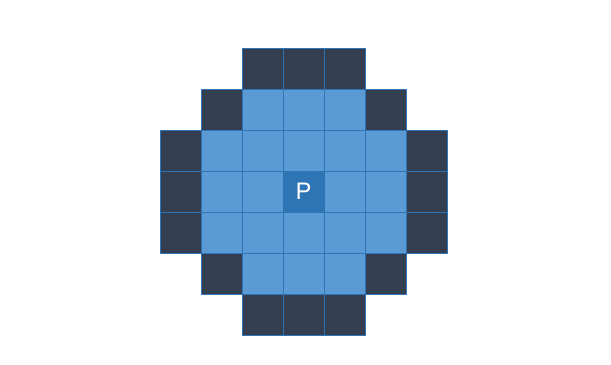
\includegraphics[width=0.5\textwidth]{FAST.png}
	\caption{FAST角点} 
	\label{fig7}
\end{figure}

% Oriented FAST
单纯的FAST关键点是不带方向性的,为了准确性,ORB的Oriented FAST关键点给FAST角点添加了方向和尺度的描述。其尺度的描述是由计算机视觉中构建金字塔模型的方法,在不同分辨率的图像下都能够提取到特征点,而旋转的描述则是由灰度质心法实现的,如图\ref{fig8}所示:

\begin{figure}[!ht]
	\centering
	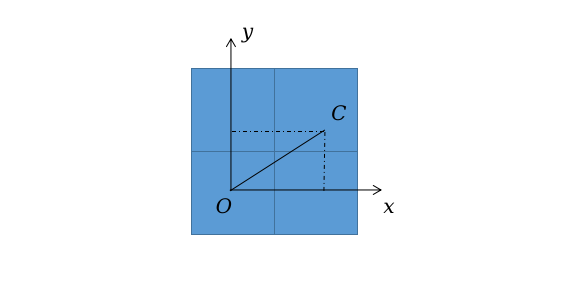
\includegraphics[width=0.5\textwidth]{OFAST.png}
	\caption{灰度质心法}
	\label{fig8}
\end{figure}

设$O$为角点像素,取一个最小的图像块,只有四个像素构成,建立$O-x-y$坐标系,原点的像素用$I(0,0)$表示,则可以找到该图像块的质心为:

\begin{equation}
C=(\frac{I(1,0)}{I(0,0)}, \frac{I(0,1)}{I(0,0)})
\end{equation}

则可以得到方向向量$\vec{OC}$,该关键点的方向定义为:

\begin{equation}
\theta = \arctan{\frac{I(0,1)}{I(1,0)}}
\end{equation}


% BRIEF
BRIEF描述子为二进制编码,反映了关键点附近128个像素对的大小关系,最终由0和1构成,其具有旋转不变性、选点速度快且易于存储。


\subsection{ORB-SLAM2的配置及运行}
% config
ORB-SLAM2是标准的CMake工程,这就意味着其可以使用CMake进行配置并且进行make编译;其虽然支持ROS,但并不是ROS的catkin工程,使用的是rosbuild相关命令,而不是ROS常见的catkin make编译指令。

ORB-SLAM2的github主页上,详细介绍了其编译的方法,官方将编译代码集成到了build.sh文件中;正常情况下,可以通过chmod +x命令给该sh文件赋予可执行权限后,运行sh命令,直接编译。如图\ref{fig10}所示,需要编译的内容为两个第三方库和ORB-SLAM2主要函数;需要注意的是,make -j命令指的是只用全部线程进行编译,这样做可能会造成电脑资源锁死,可以根据电脑的配置自行修改所用线程数。

\begin{figure}[!ht]
	\centering
	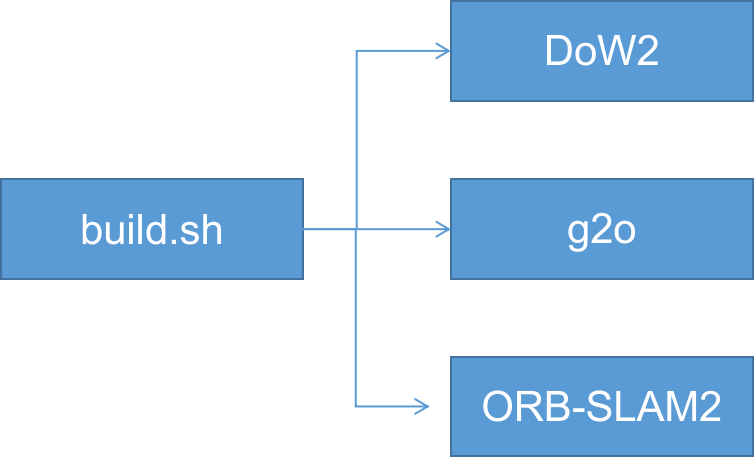
\includegraphics[width=0.45\textwidth]{build.png}
	\caption{配置ORB-SLAM2}
	\label{fig10}
\end{figure}

ORB-SLAM2在普通编译过程中,可能会遇到一些问题:
\begin{enumerate}
	\item System.cc中,usleep未定义;这是由于System.h文件中缺少头文件unistd.h导致的,加上该头文件即可。
	\item 
	找不到Eigen3库;大概率是因为Pangolin版本为0.6,但ORB-SLAM2使用的Pangolin版本为0.5;一种方法是将Pangolin版本退回0.5,另一种方法是将CMakeList.txt中的Eigen3 REQUIRED改为REQUIRED NO\_MODULE。如果仍然找不到Eigen3库,如果是用Eigen3源代码编译安装的非模板类Eigen3库,则可以通过ln -s建立软链接的方式,在ORB需要找到Eigen3的位置添加上Eigen3的库。
	\item 
	Eigen3的问题,在ROS编译的CMakeList中也需要修改。
\end{enumerate}

普通编译完成后,使用TUM数据集进行测试,从System.cc中可以得出,在终端中需要三个参数:ORB字典的路径、相机配置文件的路径、数据集的路径。

由于需要在ROS环境下使用,首先执行build\_ros.sh。之后需要添加环境变量给ROS工作空间,即在.bashrc文件中,添加上ROS功能包的路径,指向Examples/ROS文件夹。至此,ORB-SLAM2在普通环境和ROS环境下均配置完成。

ORB-SLAM2在运行时,其流程如图\ref{fig-ORBstructure}所示:
~\\
\begin{figure}[!ht]
	\centering
	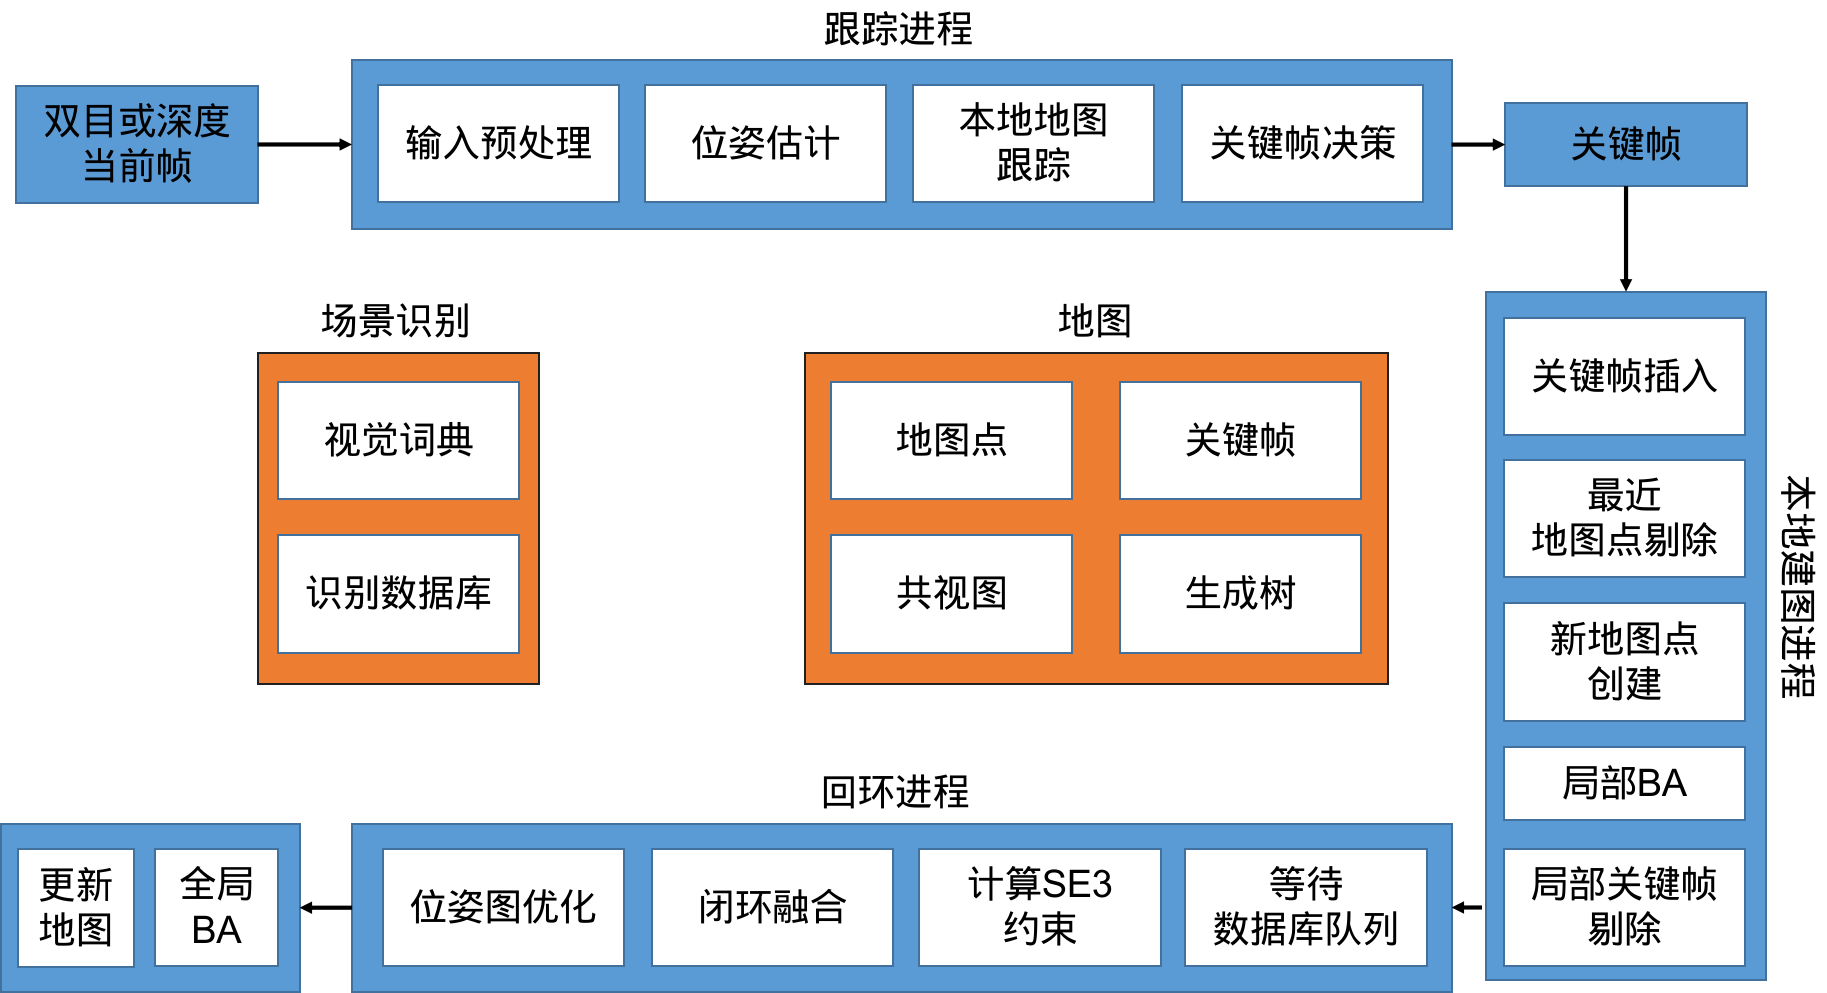
\includegraphics[width=0.94\textwidth]{ORBstructure.png}
	\caption{ORB-SLAM2整体框架}
	\label{fig-ORBstructure}
\end{figure}

\subsection{ORB-SLAM2的主要模块} \label{3.2.2}

ORB-SLAM2是一套规范完整的视觉SLAM系统,其主要进程可以分为四个:跟踪进程、本地地图进程、回环检测进程、可视化进程\cite{mur2017orb}。如图\ref{fig9}所示,从以下五个主要函数中分析。

\begin{figure}[!ht]
	\centering
	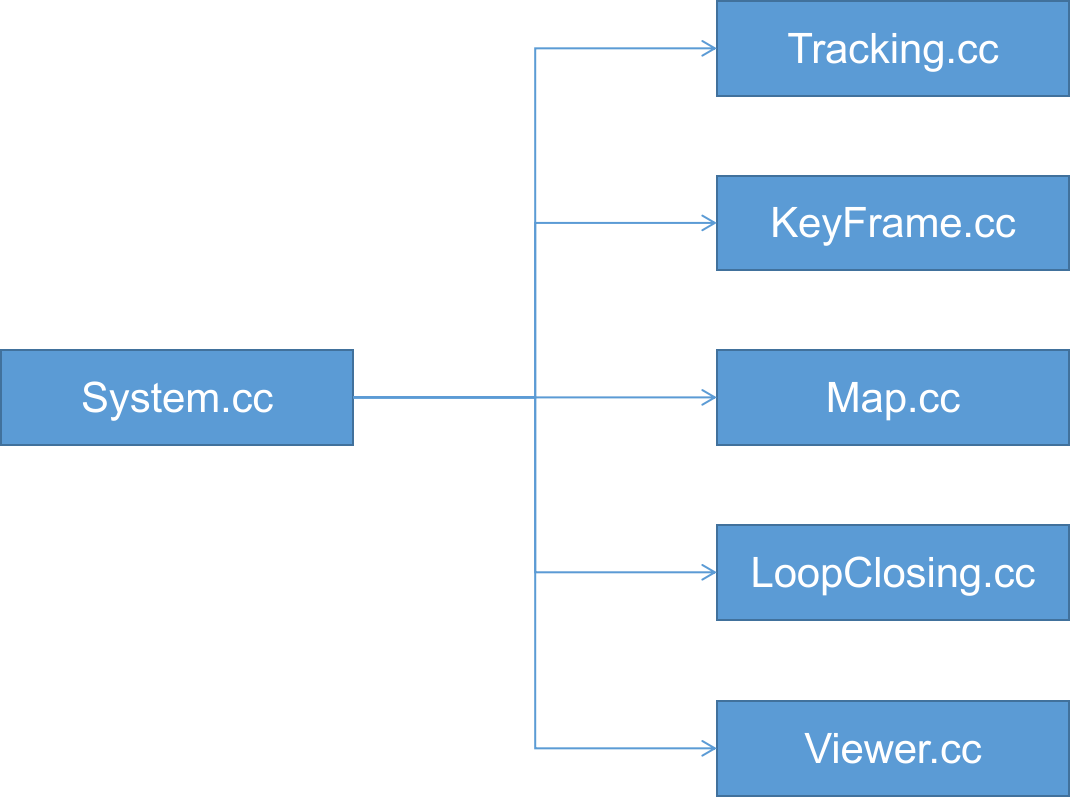
\includegraphics[width=0.65\textwidth]{ORB2.png}
	\caption{ORB-SLAM2主要模块}
	\label{fig9}
\end{figure}

% System
\textbf{System.cc},SLAM系统顶端控制:

首先是读取ORB词典,该词典是配合DoW2库训练得到的,用于回环检测时判断图像的外观相似度。

其次是创建ORB特有的KeyFrameDatabase,该类用于处理关键帧数据;创建地图,实例化Map对象;创建画笔,为可视化做准备。

\begin{minted}[fontsize=\small]{cpp}
//Create KeyFrame Database
mpKeyFrameDatabase = new KeyFrameDatabase(*mpVocabulary);

//Create the Map
mpMap = new Map();

//Create Drawers. These are used by the Viewer
mpFrameDrawer = new FrameDrawer(mpMap);
mpMapDrawer = new MapDrawer(mpMap, strSettingsFile);
\end{minted}

之后是主要线程的初始化,跟踪线程、本地地图线程和回环检测线程:
\begin{minted}[fontsize=\small]{cpp}
//Initialize the Tracking thread
//(it will live in the main thread of execution, the one that called this constructor)
mpTracker = new Tracking(this, mpVocabulary, mpFrameDrawer, mpMapDrawer,
mpMap, mpKeyFrameDatabase, strSettingsFile, mSensor);

//Initialize the Local Mapping thread and launch
mpLocalMapper = new LocalMapping(mpMap, mSensor==MONOCULAR);
mptLocalMapping = new thread(&ORB_SLAM2::LocalMapping::Run,mpLocalMapper);

//Initialize the Loop Closing thread and launch
mpLoopCloser = new LoopClosing(mpMap, mpKeyFrameDatabase, mpVocabulary, mSensor!=MONOCULAR);
mptLoopClosing = new thread(&ORB_SLAM2::LoopClosing::Run, mpLoopCloser);
\end{minted}

System相当于工程中的Main函数,汇集了实现一个SLAM系统所需的全部流程,使用顶层的代码进行控制,具体功能则由底层的类及其中的函数去实现。

% Tracking
\textbf{Tracking.cc},关键的跟踪进程,其主要函数为图像的转换函数和Track主函数:
\begin{enumerate}
	\item 
	图像转换函数是针对不同传感器设置的,以弹幕相机为例;该函数需要判断图像是否为灰度图,判断图像为RGB或BGR编码,并最后将图像转为系统使用的灰度3通道图像,赋予其时间戳和ORB字典、相机的内参矩阵和畸变参数等信息,构成当前帧的对象。
	\item 
	Track函数,该函数是Tracking.cc中的主要函数,或称之为顶端函数。该函数首先判断系统状态,之后根据状态选择使用运动模型或里程计模型得到当前位姿,以及是否需要重定位;如果得到相机位姿和正确匹配,则依次在建立的Map中跟踪路标、将路标更新到画笔中、判断是否将该帧加入关键帧、清除里程计的匹配和未跟踪的MP。
\end{enumerate}

% KeyFrame
\textbf{KeyFrame.cc},该类的操作都基于关键帧进行:

\begin{enumerate}
	\item 
	共视图;确定关键帧之间的共视关系,该内容将被用于优化及回环检测,最终建立一个关键帧之间的共视图关系。
	\item 
	地图点;还包括MP地图点的添加与移除、跟踪与匹配等;
	\item 
	位姿;包括获取位姿、旋转矩阵$\bf{R}$,平移向量$\bf{t}$等;
\end{enumerate}

% Loop Closing
\textbf{LoopClosing.cc},回环检测的主要函数:

\begin{enumerate}
	\item 检测是否有新的关键帧;在此之前要给回环的队列加互斥锁,之后返回逻辑变量,表示是否有新的关键帧;
	\item 检测是否有闭环;提取出一个关键帧,并用互斥锁加锁,防止被擦除;之后对地图进行判断,如果地图包含少于10个关键帧,则直接判定为没有闭环;使用具有共视关系的关键帧基于词袋模型进行评分,将共视关键帧得到的最高分作为最低分;最后删除其他的闭环候选帧,暂时找到与当前关键帧一致的关键帧。
	\item 计算相似变换;Sim3算法,其结果是得到两帧之间的相对位姿,只有Sim3求解器得到足够多的匹配点,才能接受该闭环帧。
	\item 融合位姿图。
\end{enumerate}



\section{CCM-SLAM}

% introduction of CCM
CCM-SLAM是由苏黎世联邦理工大学Patrik Schmuck开发,其含义是中心式协同单目视觉SLAM。
其特点是适用于多个设备(最多四个)同时运行,并且有一个终端负责管理控制和处理数据,是一种联合协同式的SLAM方案。

\subsection{CCM-SLAM的结构} \label{3.3.1}

CCM在算法上使用了ORB-SLAM2的方法,保留了其跟踪、关键帧、关键帧数据库、Sim3求解等类;与此同时,更加明确了自己的Client+Server机制,其核心是中心式的协同结构和各设备之间的通信方法。

\begin{figure}[!ht]
	\centering
	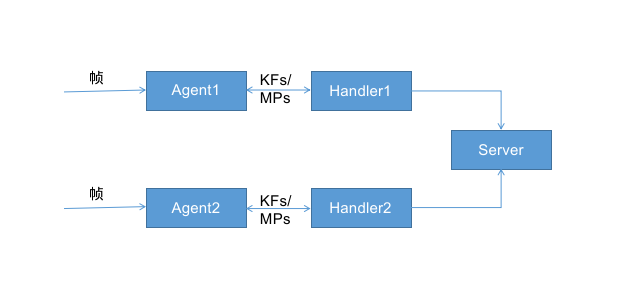
\includegraphics[width=0.6\textwidth]{CCM.png}
	\caption{CCM-SLAM框架}
	\label{fig11}
\end{figure}

% detailed CCM info
如图\ref{fig11}所示,CCM的核心是其将整个系统的SLAM进程分为了Client和Server两个模块处理。应用了网络中的客户端与服务器模型,这里的客户端指的是携带相机传感器的各设备终端,设备的种类可以是无人机、无人车、无人船甚至改进的手持相机,而服务器一般是一台中央处理电脑。

设备作为客户端,其并不是一个简单的相机加图片数据传输,而是一个有一定复杂的的运算系统。在客户端中,需要接收传感器得到的帧信息,并且做里程计运算,得到关键帧,通过通信模块将数据发送给服务器中负责接收信息的处理单元;除此之外,在客户端中还存储有建立的局部地图,地图点保持与服务器的地图数据库更新。

关键帧和地图点的数据进入服务器的信息处理单元后,地图点直接进入服务器的地图存储库中;对于新的关键帧,如果能够检测到地图场景重叠,则直接进入到优化过程,并将优化后的结果存储到地图存储库中;该关键帧正常情况下会进入地图匹配和地图融合模块,之后再进入优化环节,随后存储到库中;如果所有客户端都到达相同的场景,则最后地图存储库只会有一张地图\cite{schmuck2019ccm}。

\subsection{Client与Server机制} \label{3.3.2}

CCM-SLAM主要有两大板块的内容,一部分是地图的处理,另一部分是其客户端和服务器的机制及通讯方式。

客户端的设计可以分为三步,如图\ref{fig12}所示,整体的流程是由ClientNode到ClientSystem再到ClientHandler,其中的引用关系即为该流程。

\begin{figure}[!ht]
	\centering
	
\includegraphics[width=0.6\textwidth]{Client.png}
	\caption{Client设计}
	\label{fig12}
\end{figure}

ClientNode负责的内容包括:ROS节点初始化,句柄的设计,使用指针创建ClientSystem。在ROS节点的初始化过程中,使用的节点名称是CSLAM client node;值得注意的是其句柄的设计,一般的ROS句柄都实例化NodeHandler,但其又实例化了NodeHandler("~"),该操作旨在给相机和地图等话题之前加上节点的名称,以于不同的终端作区分;最后使用了智能指针,创建了ClientSystem对象,意味着对该客户端创建了属于其自己的客户端系统。

\begin{minted}[fontsize=\small]{cpp}
ros::init(argc, argv, "CSLAM client node");

if(argc != 3){
    cerr << "Usage: rosrun cslam clientnode path_to_vocabulary path_to_cam_params";
    ros::shutdown();
    return 1;
}

ros::NodeHandle Nh;  // topic name will be: node name(only), like "/image_raw"
// topic node will be: node name + topic name, like "iris_0/image_raw"
ros::NodeHandle NhPrivate("~"); 

boost::shared_ptr<cslam::ClientSystem> pCSys{new
                cslam::ClientSystem(Nh,NhPrivate,argv[1],argv[2])};
\end{minted}

ClientSystem负责的内容包括:读取ID,SLAM初始化及预先数据准备。首先从ROS的参数服务器读取客户端ID,使用ROS的param方法读取该数据;之后进行标准的SLAM数据预先准备流程,即加载词典、创建关键帧数据库、创建地图;最后进行初始化步骤,在这里引入了ClientHandler。

\begin{minted}[fontsize=\small]{cpp}
int ClientId;
// get ClientID from launch file, actually ROS parameter server
mNhPrivate.param("ClientId",ClientId,-1);
mClientId = static_cast<size_t>(ClientId);
// assign ClientID to member of class ClientSystem, mClientID

// load vocabulary
this->LoadVocabulary(strVocFile);

// Create KeyFrame Database
mpKFDB.reset(new KeyFrameDatabase(mpVoc));

// Create the Map
mpMap.reset(new Map(mNh,mNhPrivate,mClientId,eSystemState::CLIENT));
usleep(10000); //wait to avoid race conditions

// Initialize Agent
mpAgent.reset(new ClientHandler(mNh,mNhPrivate,mpVoc,mpKFDB,mpMap,
mClientId,mpUID,eSystemState::CLIENT,strCamFile,nullptr));
usleep(10000); //wait to avoid race conditions
mpAgent->InitializeThreads();
usleep(10000); //wait to avoid race conditions
\end{minted}

ClientHandler负责的内容包括:向总地图中添加该ID客户端的地图,定义Sim3转换,将该ID客户端的相机话题名加载到ROS的参数服务器,最后开始了具体的初始化。


\subsection{CCM-SLAM的配置}

与ORB-SLAM2相同,CCM-SLAM在其github上有详细的编译方法;与ORB-SLAM2不同的是,CCM-SLAM是完全的catkin架构,完全基于ROS,所以其必须被放置在ROS工作空间的src文件夹下,并且使用catkin make命令编译CCM-SLAM工程。需要注意的是最好不要使用全部线程进行编译。


\section{多机协同及地图融合方案}

地图的融合原理与回环检测类似,但不同于回环检测,地图融合在识别出场景重叠后,不止需要完成定位,还要对重叠场景的地图点完成归类和补充。

\subsection{算法原理} \label{3.4.1}

\begin{figure}[!ht]
	\centering
	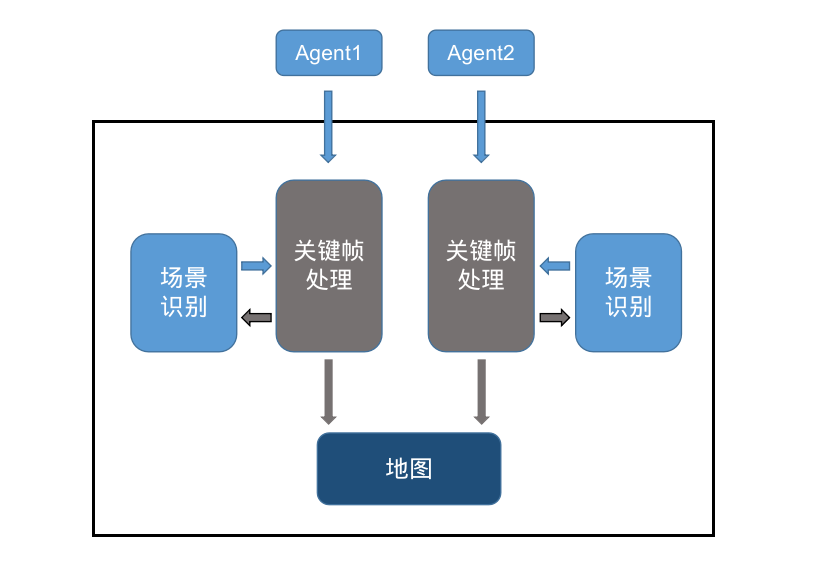
\includegraphics[width=0.6\textwidth]{csfm.png}
	\caption{系统框架}
	\label{fig13}
\end{figure}

地图融合系统的框架如图\ref{fig13}所示:无人机1和无人机2将帧信息传递给系统的关键帧处理单元,关键帧处理单元对帧做出处理,首先筛选出其中的关键帧,没有入选的帧则被舍弃。

筛选出的关键帧随后首先进入到场景识别模块,该处的作用类似回环检测,即识别出相似的场景,这一点仍然使用基于外观的相似检测,即使用BoW的词袋模型。如果没有探测到场景重叠(注意,相邻的关键帧不会被并入考虑是否重叠,除了很大概率存在重叠外,在代码的逻辑中还需剔除共视关键帧的影响),则进入正常的优化和回环检测、建图等环节;如果探测到场景重叠,则需要视情况而定\cite{forster2013collaborative}:

\begin{enumerate}
	\item 若该场景与本机已经经历过的场景重合,则不进入地图拼合模块,直接进入优化和回环检测模块;对重叠的定义需要判断是完全重叠或部分重叠,若完全重叠则也会进入到回环检测模块;若连续几帧均为部分重叠,即说明对某些点保持跟踪,而在SLAM进程中只有连续几帧都可见的路标点才会被计入地图点,属于正常跟踪进程。
	\item 若该场景与本机的场景无重合,在与另一架无人机的场景识别中探测到重叠,则会进入到地图融合进程;
\end{enumerate}

\begin{figure}[!ht]
	\centering
	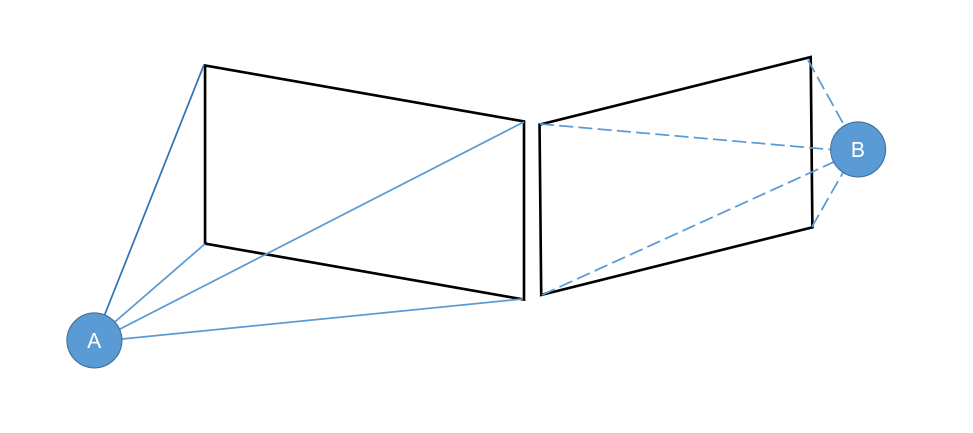
\includegraphics[width=0.6\textwidth]{theory.png}
	\caption{地图点匹配}
	\label{fig14}
\end{figure}

当确定需要地图拼合时,如图\ref{fig14}所示,将两张图像中的地图点进行特征点匹配操作;对于图中的地图点,其在两个坐标系下,通过三角测量得到的坐标是不一致的,由此推得两个坐标系的转换关系,从而以一个无人机坐标系为主,将另一个坐标系中的点进行坐标变换后,重复的点舍弃,新增的点则按照坐标系转换关系补充到地图中,从而完成地图融合。


\subsection{编程实现} \label{3.4.2}

设有四张包含场景重叠但在不同位置拍摄的图片,随机对其分为2组,一组的图片序号为1,2;二组图片的序号为3,4;

对两组图片首先进行ORB特征点提取,之后使用提取和匹配到的特征点,计算两组相机运动的位姿变换矩阵,为$T_{12},T_{34}$,则现有两套坐标转换关系,并且可以根据三角测量的方法,获得两组地图点相对于各自参考图片(1,3)的位置$P_{12},P_{34}$;

由于该场景包含重叠场景,我们默认其符合拼接地图的要求;接下来对1,3进行特征点提取和匹配,并随后计算1,3之间的转换矩阵$T_{13}$,则可以由此矩阵,将1中的地图点转换到3坐标系下:

\begin{equation}
P_{12-3}={\bf R_{13}} \times P_{12} + \bf{t_{13}}
\end{equation}

这一部分的代码实现如下,其中,shiftCoordinate函数为实现上式的函数。

\begin{minted}[fontsize=\small]{cpp}
// get KeyPoint position of Client0 in Client1
vector<Point3d> map_point0_1;
map_point0_1 = ORBMatcher::shiftCoordinate(R, t, K, map_points0);
map_point0_1.insert(map_point0_1.end(), map_points1.begin(), map_points1.end());
// show combination map
ORBMatcher::showMapPoints(map_point0_1);

vector<cv::Point3d> ORBMatcher::shiftCoordinate(const Mat &R, const Mat &t, const Mat &K,
const vector<cv::Point3d> &pos) {
    // Pos_new = (RP + t)
    vector<Point3d> shiftedPos;
    Point3d p;

    Eigen::Matrix<double, 3, 3> Mat_R;
    Eigen::Matrix<double, 3, 1> Mat_t;
    Eigen::Matrix<double, 3, 1> Mat_P;
    Eigen::Matrix<double, 3, 3> Mat_K;
    Eigen::Matrix<double, 3, 1> Mat_Pos;

    cv2eigen(R, Mat_R);
    cv2eigen(t, Mat_t);

    for (const auto & po : pos){
        Mat_Pos << po.x, po.y, po.z;
        Mat_P = Mat_R * Mat_Pos + Mat_t;
        p.x = Mat_P(0);
        p.y = Mat_P(1);
        p.z = Mat_P(2);
        shiftedPos.push_back(p);
    }
    return shiftedPos;
}
\end{minted}

实现点云绘制的为showMapPoints函数,主要使用了Pangolin库,使用OpenGL对各点进行绘制并且给出可交互窗口。其中的关键循环如下:

\begin{minted}[fontsize=\small]{cpp}
for (const auto & MapPoint : MapPoints){
    glVertex3d(MapPoint.x, MapPoint.y, MapPoint.z);
}
\end{minted}

由此获得了简单的拼合场景;

\begin{figure}[htbp]
	\centering
	\begin{minipage}[t]{0.45\columnwidth} %小于1/n如果使用n张图片
		\centering
		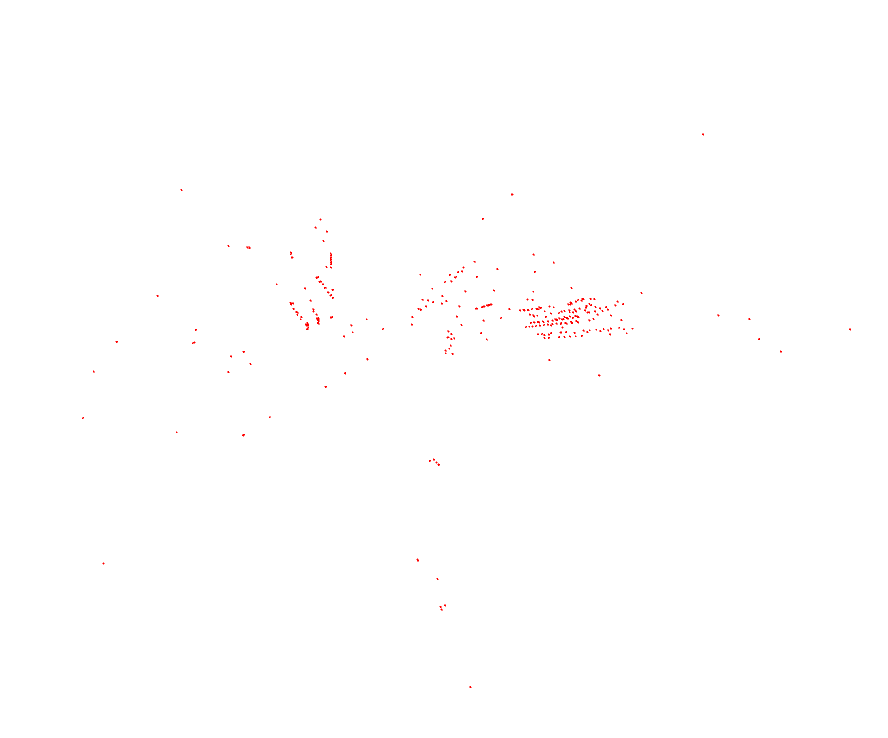
\includegraphics[width=0.8\columnwidth]{merge3.png}
		\caption{单独地图点}
		\label{merge1}
	\end{minipage}
	\begin{minipage}[t]{0.45\columnwidth}
		\centering
		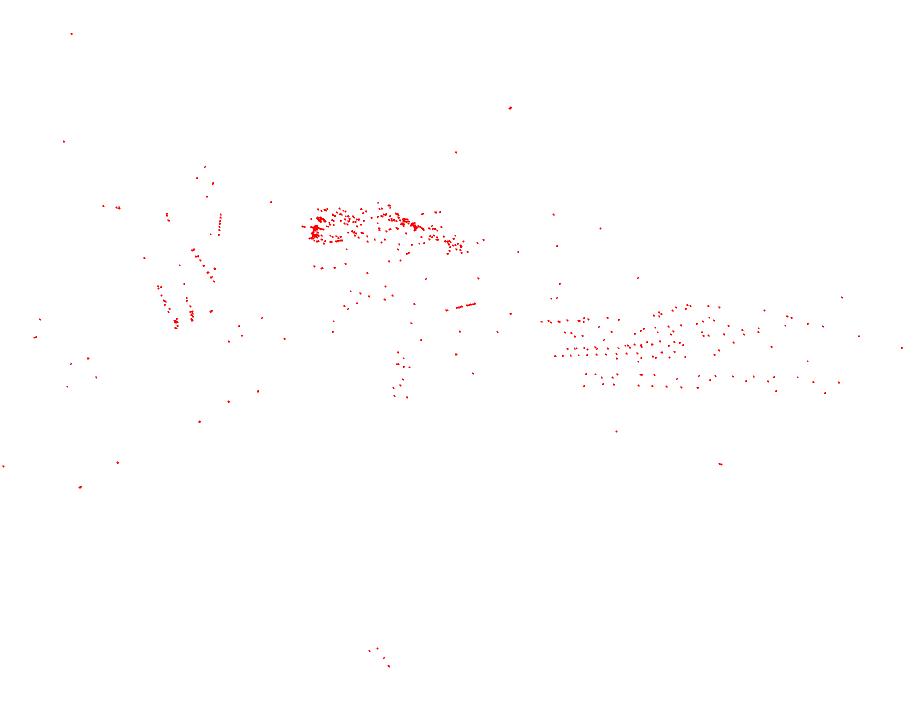
\includegraphics[width=0.8\columnwidth]{merge4.png}
		\caption{合并地图点}
		\label{merge2}
	\end{minipage}
\end{figure}










\chapter{多无人机SLAM仿真} \label{Simulation}

% 介绍框架
本章主要多无人机SLAM的仿真;为了循序渐进,首先介绍仿真环境的配置,其次是单机的SLAM仿真,最后过渡到多机的SLAM仿真。


\section{gazebo仿真环境配置}

在进行仿真之前,首先要对场景进行搭建,对launch文件进行配置。

\subsection{场景} \label{4.1.1}

仿真环境中,场景的设计不能过于简单,墙壁、地面等大面积重复物体应该具有纹理,否则ORB-SLAM2的特征点提取会十分困难;除了纹理的设计,还应尽可能多地提供物体,使场景丰富。如图\ref{fig3-1}所示:

\begin{figure}[!ht]
	\centering
	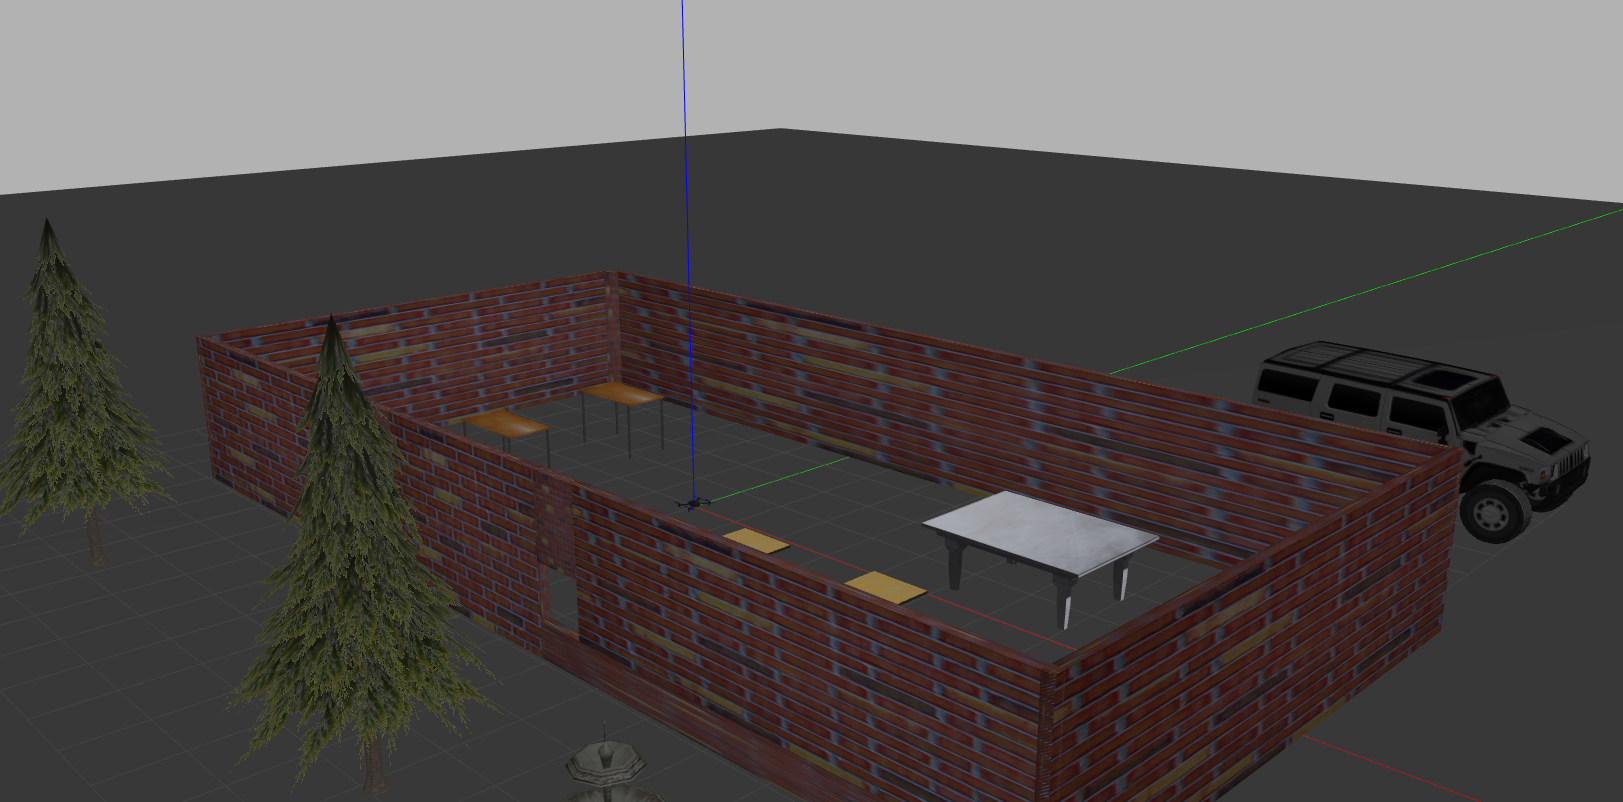
\includegraphics[width=0.7\textwidth]{scene.png}
	\caption{gazebo场景示例}
	\label{fig4-1}
\end{figure}

进入gazebo界面后,使用Control+B进入其编辑界面;之后有两种选择:

\begin{enumerate}
	\item 建立基础模型,一般在这里会绘制上地面及其纹理;如果是室内场景,还会绘制一个大致的墙壁结构,墙壁的纹理,其上的门窗等;最后将该模型保存到.gazebo/model文件中,这是gazebo模型的默认文件。
	\item 直接选择插入模型;可以在此直接插入上文建立的基础模型,也可以插入其他模型库已有的模型,默认存储在/.gazebo/models文件夹下
\end{enumerate}

最后需要将自建场景存储为一个.world文件,gazebo不会给文件后缀的提示,需要自己输入后缀,这一点需要特别注意。在此之后,就获得了自建的world场景,下一步需要在launch文件中更改该项,完成调用。


\subsection{launch文件} \label{4.1.2}

\ref{2.1.2}节中,曾简单介绍launch文件的功能。作为整个仿真环境的配置文件,launch文件中基本包含了仿真所需的参数。

launch文件使用XML标签语言书写,主要为确定启动的节点和加载参数使用,简单的开始节点、加载参数的方法如下:

\begin{lstlisting}[language={XML}]
<node pkg="your package name" name="your node name" type="your node type"/>
<param name="param name" value="param value"/>
<arg name="arg name" default="arg value"/>
\end{lstlisting}

在一个简单的launch文件中,主要会包括设备的信息设置、PX4配置和gazebo仿真配置。

\begin{enumerate}
	\item 设备的信息设置;这一部分包括设备的位姿,通过$x,y,z,R,P,Y$6个变量表示三维位置坐标和滚转、俯仰、偏航姿态角;还包括设置设备的类型和名称,在四旋翼无人机仿真中使用iris作为参数vehicle的值,并且在sdf参数中,将sdf参数的值指向iris的sdf文件(一般在该位置,都使用默认参数加find指令去寻找软件在环仿真的gazebo模型路径);最后是一些gui等参数的设置,默认使用官方设置的即可。
	\item PX4软件在环仿真的参数;在这里启动了名为sitl的节点,其参数指向了EKF设置的rcS文件;
	\item gazebo仿真参数配置;在这里需要修改world\_name参数,其默认是world参数的值,所以实际上也可以直接修改world参数值,将其指向自建的world文件。
\end{enumerate}

自此,launch文件配置完成,可以使用PX4启动launch文件来进行简单的仿真。


\section{单机SLAM仿真}

在进行多机仿真前,首先要进行单机的SLAM仿真,为多机仿真做铺垫。单机SLAM仿真分为单机Offboard模式起降和航路点飞行,以及SLAM下的起降和航路点飞行四步。

\subsection{launch文件配置} \label{4.2.1}

\ref{4.1.2}节中介绍了launch文件的详细配置方法,对于单机的SLAM仿真,配置方法基本与其相同,但是需要给iris无人机假装上双目相机。以下介绍给无人机加装相机的方法:

选择mavros\_posix\_sitl.launch文件,找到设备模型和世界配置区块,原始设置如下:

\begin{lstlisting}[language={XML}]
<!-- vehicle model and world -->
<arg name="est" default="ekf2"/>
<arg name="vehicle" default="iris"/>
<arg name="world" default="$(find mavlink_sitl_gazebo)/worlds/empty.world"/>
<arg name="sdf" default="$(find mavlink_sitl_gazebo)/models/$(arg vehicle)/$(arg vehicle).sdf"/>
\end{lstlisting}

加载双目相机,也就是给iris无人机装上相机,需要在设备配置处,加上其附加配置的sdf文件;由于在这里只添加了相机的sdf文件,所以该附加sdf文件不需要手动修改,直接链接到相机上即可。因此需要新建camera参数,其值为iris\_stereo\_camera,是gazebo自带的可以添加到iris无人机上的双目相机,修改后的launch文件部分如下:

\begin{lstlisting}[language={XML}]
<!-- vehicle model and world -->
<arg name="est" default="ekf2"/>
<arg name="vehicle" default="iris"/>
<!-- add stereo camera for iris -->
<arg name="my_camera" default="iris_stereo_camera"/>
<arg name="world" default="$(find mavlink_sitl_gazebo)/worlds/empty.world"/>
<!-- also need to revise sdf -->
<arg name="sdf" default="$(find mavlink_sitl_gazebo)/models/$(arg my_camera)/$(arg my_camera).sdf"/>
<!-- <arg name="sdf" default="$(find mavlink_sitl_gazebo)/models/$(arg vehicle)/$(arg vehicle).sdf"/> -->
\end{lstlisting}

更改完launch文件的无人机配置后,可以试运行来检测,即roslaunch该launch文件。之后有两种方法可以检查,一是使用rostopic list命令,查找当前活跃的话题,如果MAVROS能顺利连接上双目相机,则会出现image\_raw话题(对于双目分为左右,但对于单目仅有一个话题),这种情况下一般是成功的;另一种方法是使用ROS自带的rqt\_graph命令,该命令可以以图的形式展示出,这种方式用途更广。装配成功后,仿真加载时应如图\ref{fig4-2}所示:

% 或许可以加一张大图

\begin{figure}[!ht]
	\centering
	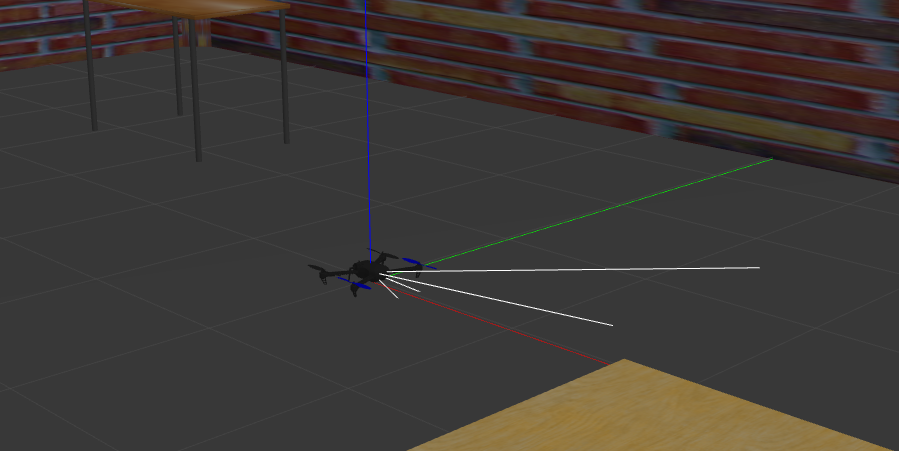
\includegraphics[width=0.7\textwidth]{mono_uav.png}
	\caption{装配相机的iris无人机}
	\label{fig4-2}
\end{figure}

需要注意,在需要与MAVROS建立通信的launch文件中,需要设置fcu端口号,具体表示为udp+本地端口号,在多机的launch文件中,每一架飞机的端口号都是不同的,但单机不需要作出修改。

如果设置双目相机参数后加载失败或加载到一个正方体模型,则是双目相机模型缺失导致的。一种方法是删除gazebo自带的models中的双目相机,并用PX4中的双目相机模型代替;另一种方法则是直接将sdf的值指向PX4的双目相机,即其值为PX4双目相机的路径。

\subsection{Offboard程序} \label{4.2.2}

完成双目相机的配置后,第二步是进入Offboard程序。与\ref{2.2.3}的Offboard模式类似,首先目标是完成一套完整的起飞降落。需要注意,Offboard模式中,所有消息指令都需要以大于$2Hz$的频率发送,否则会激活安全生效机制,飞机返航。

\begin{enumerate}
	\item 起飞的方式。动力学模型上的起飞即给四旋翼增加动力,保持平衡并提供向上的大于重力的升力,在程序中表示为发布位置指令,该消息类型为MAVROS的geometry\_msgs数据类型。
	\item 降落的方式。一般使用切换飞行模式的方法,将飞行模式切换到降落模式,选择降落模式中的自动降落即可。
\end{enumerate}

降落的程序如下:

\begin{lstlisting}[language={C++}]
// proceed landing process
ROS_INFO("landing");
mavros_msgs::SetMode land_set_mode;
land_set_mode.request.custom_mode = "AUTO.LAND";
while (ros::ok()){
if( current_state.mode != "AUTO.LAND" &&
(ros::Time::now() - last_request > ros::Duration(5.0))){
if( set_mode_client.call(land_set_mode) &&
land_set_mode.response.mode_sent){
ROS_INFO("Land enabled");
}
last_request = ros::Time::now();
}
if(!current_state.armed){
break;
}

ros::spinOnce();
rate.sleep();
}
\end{lstlisting}

航路点飞行的简单实现方法为,依次发布各航路点的位置信息,但需要一个函数去判断飞机是否到达了航路点。函数的实现可以利用预计坐标和现处位置之间的欧式距离作评判标准,小于某值则认为到达航路点,实现的关键在现处位置消息的订阅。首先需要定义current\_pose作为现处位置的变量,之后定义回调函数,获得该信息,实现的代码如下:

\begin{lstlisting}[language={C++}]
// record current pose
geometry_msgs::PoseStamped current_pose; /* NOLINT */

// callback function for Subscriber for local_pos_sub
void local_cb(const geometry_msgs::PoseStamped::ConstPtr& msg){
current_pose = *msg;
}
\end{lstlisting}

检查是否到达航路点的函数如下:

\begin{lstlisting}[language={C++}]
// check if reached a waypoint
bool check_waypoint(const geometry_msgs::PoseStamped &now_pose, const geometry_msgs::PoseStamped &aim_pose){
// define Point to hold current position and aim position
geometry_msgs::Point curr, aim;
curr = now_pose.pose.position;
aim = aim_pose.pose.position;
double precision = 0.1;

// define return value
bool reach = false;

// calculate distance
double dist = sqrt(pow((curr.x - aim.x), 2) +
pow((curr.y - aim.y), 2) + pow((curr.z - aim.z), 2));
if(dist < precision){
reach = true;
ROS_INFO("reached waypoint!");
}

return reach;
}
\end{lstlisting}

前往下一个航路点的方法如下:

\begin{lstlisting}[language={C++}]
// set second waypoint
geometry_msgs::PoseStamped pose2;
pose2.pose.position.x = 2;
pose2.pose.position.y = 2;
pose2.pose.position.z = 2;

// heading for waypoint 2
while(ros::ok()){
// publish pose1 information
local_pos_pub.publish(pose2);
ros::spinOnce();

// check if reached a waypoint
if (check_waypoint(current_pose, pose2)) break;
rate.sleep();
}
\end{lstlisting}

按2个航路点飞行的地面站轨迹示意图如图\ref{fig4-3}所示:

\begin{figure}[!ht]
	\centering
	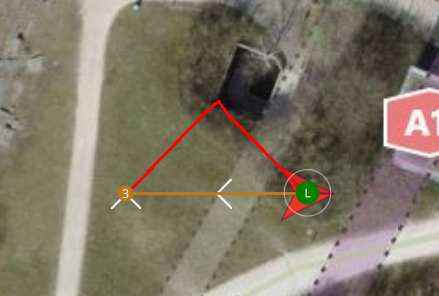
\includegraphics[width=0.6\textwidth]{waypoint.png}
	\caption{地面站的航路点飞行轨迹}
	\label{fig4-3}
\end{figure}

\subsection{视觉定位的坐标变换} \label{4.2.3}

在正常GPS定位的Offboard模式下,飞机的位置在MAVROS中作为已知量存在。但在视觉定位模式下,MAVROS需要通过vision\_pose/pose话题获得飞机的位姿信息。而ORB-SLAM2解算出的位姿并不是MAVROS的地理位置消息格式,因此需要做一些转换。

\begin{figure}[!ht]
	\centering
	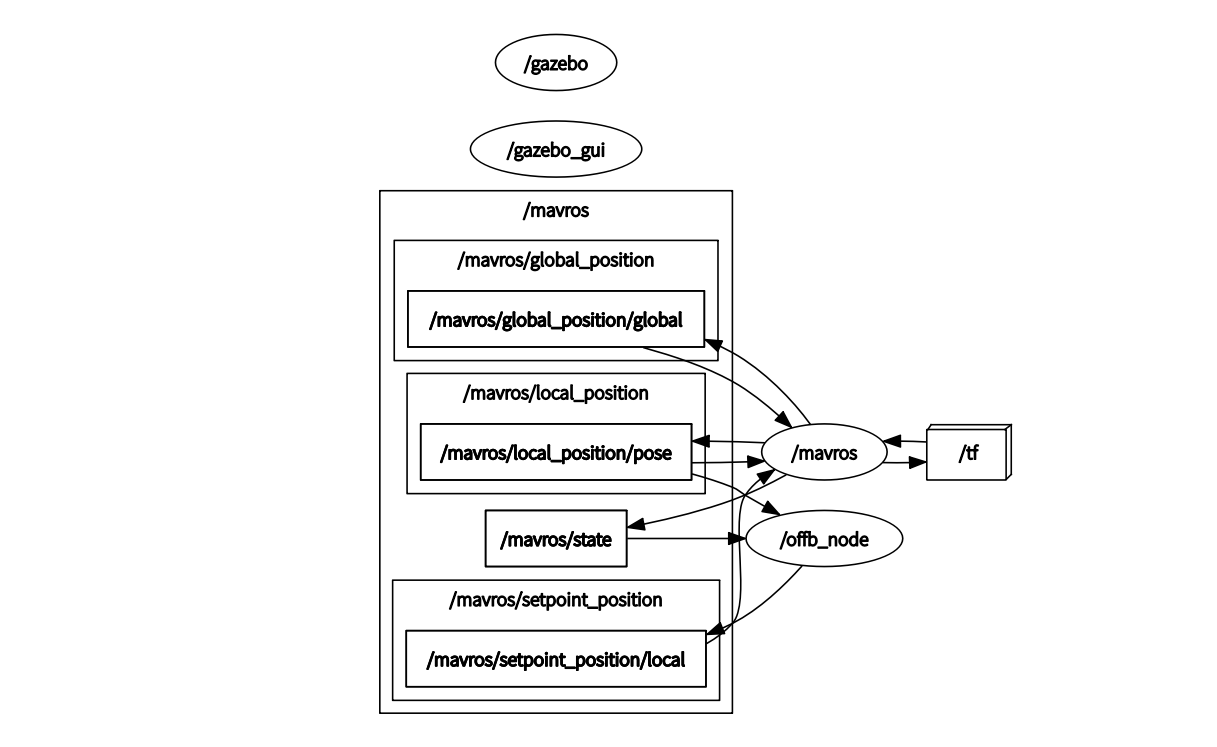
\includegraphics[width=0.8\textwidth]{rqtOffboard.png}
	\caption{Offboard节点话题关系}
	\label{fig4-4}
\end{figure}

\begin{figure}[!ht]
	\centering
	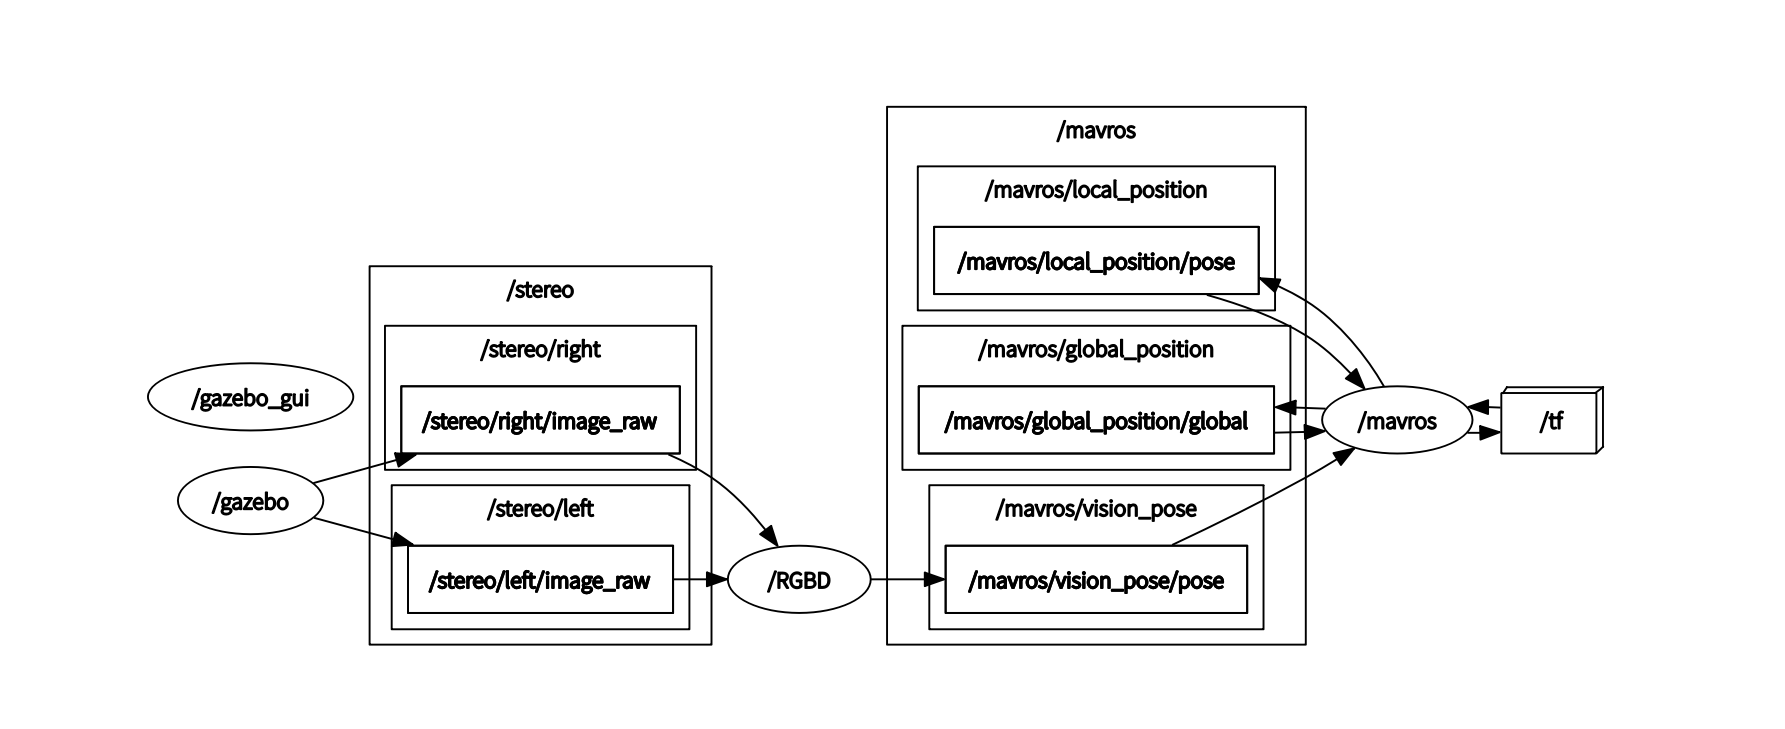
\includegraphics[width=0.4\textwidth]{rqtRGBD.png}
	\caption{视觉SLAM节点话题关系}
	\label{fig4-5}
\end{figure}

ORB-SLAM2得到的外参$\bf{Tcw}$矩阵为$4 \times 4$矩阵:

$$
\bf{Tcw}=\begin{bmatrix}
\bf{R_{cw}} & \bf{t_{cw}}\\0 & 1
\end{bmatrix}
$$
其中,$\bf{R_{cw}}$为旋转矩阵,$\bf{t_{cw}}$为平移向量。

可以证明,从相机的外参矩阵得到相机位姿:

$$
\begin{aligned}
\bf{R_{wc}}= &\bf{R_{cw}}^T\\
\bf{t_{wc}}= &-\bf{R_{wc}} \cdot  \bf{t_{cw}}
\end{aligned}
$$

在此之后,还需要将$\bf{R_{wc}}$和$\bf{t_{wc}}$赋值给ROS中tf坐标系类型的Transform变量,之后通过调用ROS的poseTFToMsg函数,将tf类型的变量转为MAVROS的地理位置消息类型变量。实现的代码如下:

\begin{lstlisting}[language={C++}]
Rwc = Tcw.rowRange(0,3).colRange(0,3).t(); // Rotation information
twc = -Rwc*Tcw.rowRange(0,3).col(3); // translation information
vector<float> q = ORB_SLAM2::Converter::toQuaternion(Rwc);

tf::Transform new_transform;
new_transform.setOrigin(tf::Vector3(twc.at<float>(0, 0), twc.at<float>(0, 1), twc.at<float>(0, 2)));

tf::Quaternion quaternion(q[0], q[1], q[2], q[3]);
new_transform.setRotation(quaternion);

tf::poseTFToMsg(new_transform, pose.pose);
x = pose.pose.position.x;
y = pose.pose.position.y;
z = pose.pose.position.z;
pose.pose.position.x = z;
pose.pose.position.y = -x;
pose.pose.position.z = -y;
orb_pub->publish(pose);
\end{lstlisting}

\subsection{单机仿真实验结果} \label{4.2.4}

% 多补充几张图

进行起飞后SLAM建图的结果:

\begin{figure}[!ht]
	\centering
	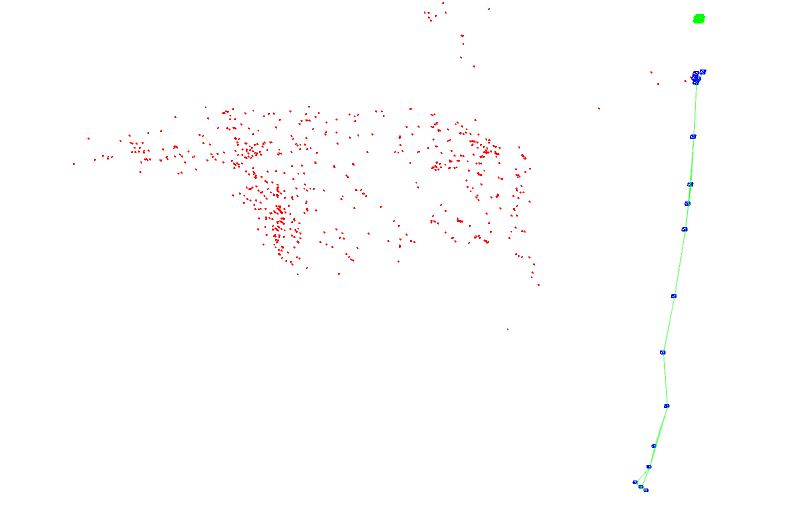
\includegraphics[width=0.4\textwidth]{single.png}
	\caption{单机SLAM的效果}
	\label{fig4-6}
\end{figure}




\section{多机SLAM仿真}


\subsection{launch文件配置} \label{4.3.1}

多机配置与单机配置最大的区别是,引用的子文件不同;单机引用posix\_sitl文件,而多机则引用vehicle\_spawn文件,而spawn文件是多机所独有的。

进入多机的launch文件,则需要引入组的概念。一个组使用一个命名空间,具有一套MAVROS的配置信息,多个组可以并行存在。因此在多机的launch文件设计中,一个组就是一架飞机,需要设置该组的命名空间,该组下的所有话题将共同使用该命名空间开头的话题。除此之外,还需要修改无人机的ID,ID默认从0到10;之后修改fcu地址和MAVLINK的udp端口,一般在末尾加上该无人机的ID即可。完整的双机launch配置代码如下:

\begin{lstlisting}[language={XML}]
<!-- UAV0 -->
<group ns="uav0">
<!-- MAVROS and vehicle configs -->
<arg name="ID" value="0"/>
<arg name="fcu_url" default="udp://:14540@localhost:14580"/>
<!-- PX4 SITL and vehicle spawn -->
<include file="$(find px4)/launch/single_vehicle_spawn_rcs.launch">
<arg name="x" value="0"/>
<arg name="y" value="0"/>
<arg name="z" value="0"/>
<arg name="R" value="0"/>
<arg name="P" value="0"/>
<arg name="Y" value="0"/>
<arg name="vehicle" value="$(arg vehicle)"/>

<arg name="my_camera" value="iris_fpv_cam"/>

<arg name="mavlink_udp_port" value="14560"/>
<arg name="mavlink_tcp_port" value="4560"/>
<arg name="ID" value="$(arg ID)"/>
<arg name="gst_udp_port" value="$(eval 5600 + arg('ID'))"/>
<arg name="video_uri" value="$(eval 5600 + arg('ID'))"/>
<arg name="mavlink_cam_udp_port" value="$(eval 14530 + arg('ID'))"/>


</include>
<!-- MAVROS -->
<include file="$(find mavros)/launch/px4.launch">
<arg name="fcu_url" value="$(arg fcu_url)"/>
<arg name="gcs_url" value=""/>
<arg name="tgt_system" value="$(eval 1 + arg('ID'))"/>
<arg name="tgt_component" value="1"/>
</include>
</group>

<!-- UAV1 -->
<group ns="uav1">                              
<!-- MAVROS and vehicle configs -->
<arg name="ID" value="1"/>
<arg name="fcu_url" default="udp://:14541@localhost:14581"/>
<!-- PX4 SITL and vehicle spawn -->
<include file="$(find px4)/launch/single_vehicle_spawn_rcs.launch">
<arg name="x" value="2"/>
<arg name="y" value="0"/>
<arg name="z" value="0"/>
<arg name="R" value="0"/>
<arg name="P" value="0"/>
<arg name="Y" value="0"/>
<arg name="vehicle" value="$(arg vehicle)"/>

<arg name="my_camera" value="iris_fpv_cam"/>

<arg name="mavlink_udp_port" value="14561"/>
<arg name="mavlink_tcp_port" value="4560"/>
<arg name="ID" value="$(arg ID)"/>
<arg name="gst_udp_port" value="$(eval 5600 + arg('ID'))"/>
<arg name="video_uri" value="$(eval 5600 + arg('ID'))"/>
<arg name="mavlink_cam_udp_port" value="$(eval 14530 + arg('ID'))"/>


</include>
<!-- MAVROS -->
<include file="$(find mavros)/launch/px4.launch">
<arg name="fcu_url" value="$(arg fcu_url)"/>
<arg name="gcs_url" value=""/>
<arg name="tgt_system" value="$(eval 1 + arg('ID'))"/>
<arg name="tgt_component" value="1"/>
</include>
</group>
\end{lstlisting}

其默认每架无人机调用的是spawn文件,其中关键的模型组合有两种方式,一种是使用urdf进行模型配置,一种是使用新的sdf。具体使用哪种视PX4的版本而定,由于urdf模型的配制方法要旧于sdf,新版的PX4统一使用sdf进行gazebo仿真的模型配置,并且使用jinja.py脚本生成sdf模型配置。

\begin{figure}[!ht]
	\centering
	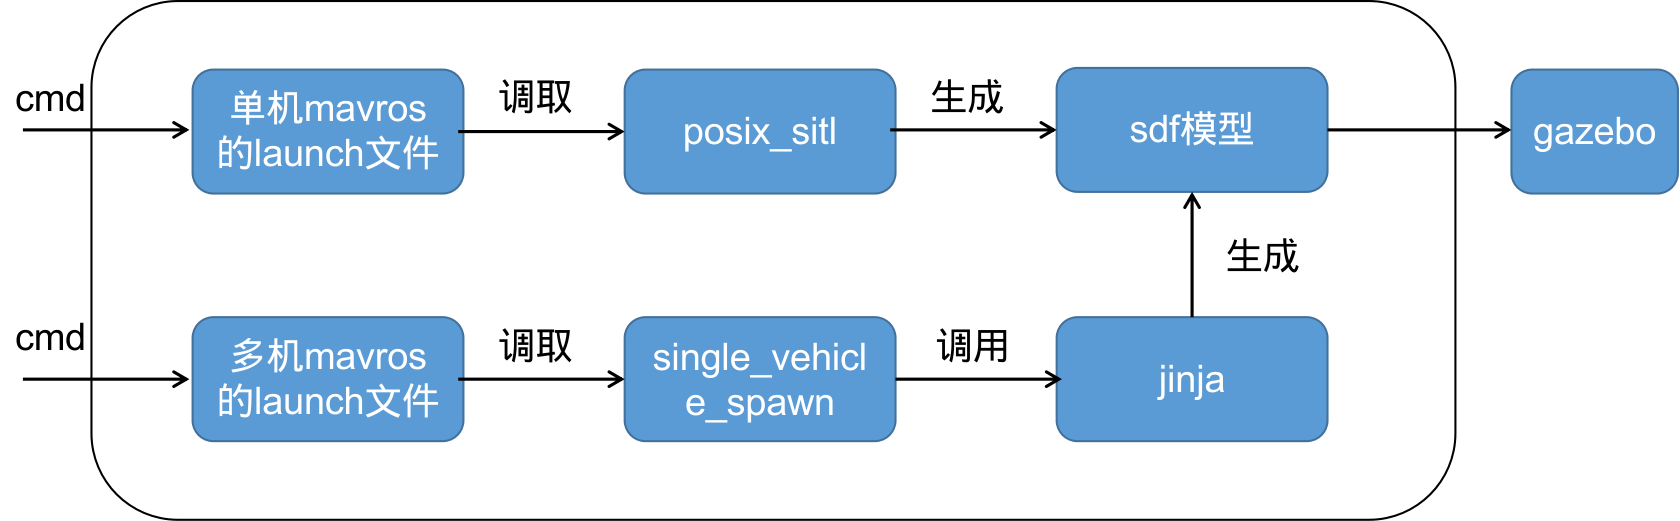
\includegraphics[width=0.8\textwidth]{sdf.png}
	\caption{仿真模型生成流程}
	\label{fig-sdf}
\end{figure}

图\ref{fig-sdf}展示了PX4中使用gazebo生成模型的方法,决定了修改模型的方法。可以看出,launch文件分为顶层和底层文件;平常直接使用roslaunch命令启动的一般为顶层文件,而顶层文件中调取的一般为底层文件。对于单机和多机,其调用的底层文件不同;单机调取posix\_sitl.launch文件,而多机则调取single\_vehicle\_spawn文件。二者的区别是单机的底层文件直接使用了即有的sdf模型,但多机的底层文件基于spawn繁殖机制,重新调用jinja生成了新的sdf模型,并且在该过程中对MAVLINK的许多参数作了配置,这一点是单机所没有的。最终都生成gazebo可以加载出的模型文件。

旧版本使用urdf版本的PX4,如果在launch文件中直接将其修改为sdf格式生成的模型,一般会报错jinja.py文件中有很多参数未定义,一种简单的处理方式是直接将新版本的janja替换到旧版本中去(为什么要使用旧版本,因为新版本的稳定性可能存在一些问题),但是这样做可能会连带产生一些附加问题,尽量选择不修改jinja这种较为底层的文件。

由于ROS的机制,话题如果重复,则会报错,并用时间戳最新的话题替换掉时间戳更旧的话题;如果多架无人机的话题不加以区分,可能会导致最终话题重复,从而只有一架无人机可以使用。


\subsection{多机编队处理} \label{4.3.2}

多机的控制可以使用编队控制,控制方法可以分为两种:集中式和分布式。

\begin{enumerate}
	\item 集中式即集群中存在领机,其他飞机需要跟随领机的运动轨迹。这种方式的实现相对简单,需要各机实时订阅领机的位置,并且始终和领机保持设定好的队形,也就是相对位置。
	\item 分布式则没有领机的概念,各无人机按照各自设定好的航路点行进,该方式的实现方法主要需要依靠多线程的设计。
\end{enumerate}

当无人机数量较多时,可以采用分级跟随的办法,假设有N架无人机,则构建一个$N \times N$邻接矩阵$T$,这里以$N=5$为例:

$$
T=\begin{bmatrix}
0 & 0 & 0 & 0 & 0\\
1 & 0 & 0 & 0 & 0\\
1 & 1 & 0 & 0 & 0\\
0 & 1 & 1 & 0 & 0\\
0 & 0 & 1 & 1 & 0
\end{bmatrix}
$$

若$N_{i,j}>0$,则$i,j$之间会建立通信,如图\ref{fig4-7}所示:

\begin{figure}[!ht]
	\centering
	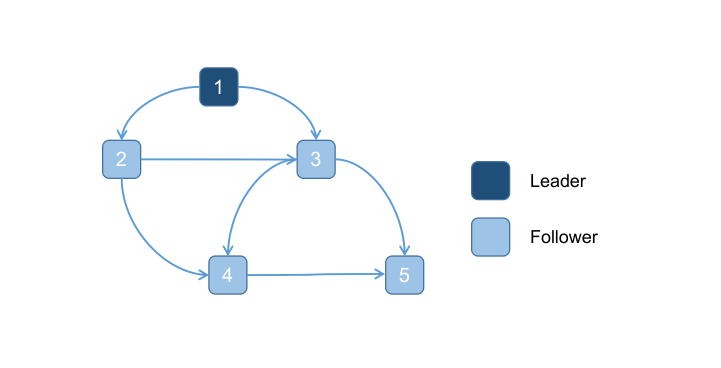
\includegraphics[width=0.6\textwidth]{formation.png}
	\caption{编队通信方法}
	\label{fig4-7}
\end{figure}

有$N_{2,1},N_{3,1},N_{3,2},N_{4,2},N_{4,3},N_{5,3},N_{5,4}$均不为0,则在这些对之间,按由小到大的顺序建立通信,传输长机的位置信息,保持相对位置的跟随。

在无人机发生编队队形变换时,则需要考虑最小总路径,可以用KM匈牙利算法解得每一架飞机对应的最小路径,并且在队形变换过程中需要考虑碰撞的影响。

图\ref{fig4-8}展示了三机编队的仿真结果:

\begin{figure}[!ht]
	\centering
	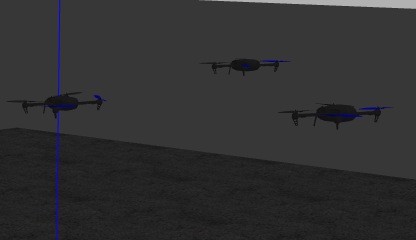
\includegraphics[width=0.5\textwidth]{multi.png}
	\caption{三机编队仿真}
	\label{fig4-8}
\end{figure}




\subsection{多机SLAM仿真} \label{4.3.3}

多机SLAM仿真除PX4的配置外,还要对SLAM的launch文件进行配置。其中包含了设置相机的参数文件,更重要的是配置各无人机所接受的相机话题。

\begin{lstlisting}[language={XML}]
<?xml version="1.0"?>
<launch>

<arg name="dist" default="0"/>
<arg name="cam" default="$(find ccmslam)/conf/px4_sitl.yaml"/>

<group ns="ccmslam">

<node pkg="tf" type="static_transform_publisher" name="linkC0_broadcaster" args="-100 300 5 -1.571 0 -2 world odomC0 100" /> 

<node pkg="ccmslam" type="ccmslamClientNode" name="ccmslamClientNode0" args="$(find ccmslam)/conf/ORBvoc.txt $(arg cam)" output="screen">

<!-- ++++++++++++++++++++++++++++++++++++++++++++++ -->
<!-- Agent Specific Params - !!!MUST BE ADJUSTED!!! -->

<param name="~FrameId" type="string" value="odomC0" />
<param name="~ClientId" type="int" value="0" />

<param name="~TopicNameCamSub" type="string" value="/iris0/usb_cam/image_raw" />

<param name="~MapInTopicName" type="string" value="MapOutServer0" unless="$(arg dist)" />
<param name="~MapInTopicName" type="string" value="MapOutServer0Disturbed" if="$(arg dist)" /> 

</node>

</group>
</launch>
\end{lstlisting}

启动时需要启动服务器和客户端,然后打开ORB-SLAM节点,最终结果如图:

\begin{figure}[!ht]
	\centering
	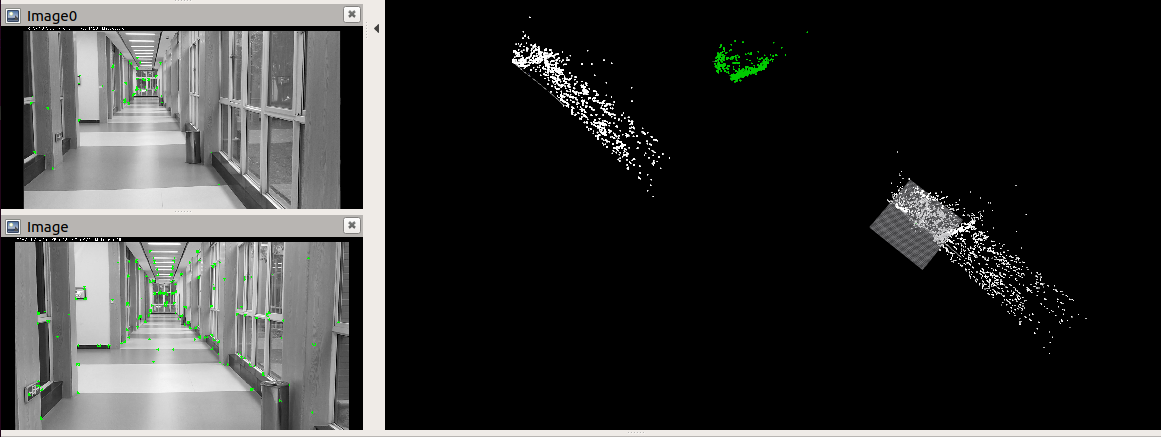
\includegraphics[width=0.9\textwidth]{ccm1.png}
	\caption{多机仿真结果}
	\label{fig4-9}
\end{figure}




































\chapter{实验与评估} \label{experiment}

进行的实验主要有两部分,真机的SLAM实验和地图融合实验。

\section{真机配置与实验}

真机使用单机实验。

真机搭载英特尔T265摄像头,其特点是带两个鱼眼镜头和惯性测量单元,并且视觉SLAM可以运行在其特有的视觉处理单元上。其在电脑上需要一定配置,安装英特尔的一些以来库文件和realsense-viewer。

除摄像头外,真机还搭载Jetson Xavier NX计算机,体积较小且接口丰富。需要注意的是,无人机在地面时,可以使用显示器和鼠标设备对其进行操作,运行ROS节点;但当无人机在空中时,没有显示信息和鼠标的操作输入,因此需要使用远程控制,在这里使用了No Machine软件进行远程控制。

实验内容;



\section{地图融合实验}

在教学楼楼道场景下,使用手持相机的方式,沿楼道行走,完成对一段楼道的建图;同时准备另一台相机,沿不同的路线行进,完成对同一段楼道的建图;两段视频应该拥有一部分重合的场景和一部分不重合的场景,用以验证地图融合的效果。

需要注意的是,使用单目视觉SLAM时,初始化是一个重要的步骤,一般采用在一个场景左右平移的方法完成初始化,之后才能进行跟踪进程,否则一段视频中将会有大量的时间用于初始化,这也意味着选取视频的质量十分重要。

在进行SLAM进程前,需要对相机进行标定,可以采用张正友标定法;需要注意的是,相机的拍照模式和录像模式,其内参矩阵可能不同;对于使用视觉SLAM的相机,建议采用动态标定法。

最后,使用预先录制的视频验证SLAM算法有两个方式:

\begin{enumerate}
	\item 将视频转换成KITTI或TUM数据集的格式;通过观察这些数据集的格式可以看出,其一般是灰度图加深度信息,并且配有时间戳,这样的转换可能有一些复杂。转换完成后,使用ROS的例子中自带的对于特定传感器和特定数据集的可执行文件运行整个SLAM进程即可。
	\item 较为简单的方式是将其转换为ROS的rosbag,rosbag可以记录特定话题的信息;对于视频而言,即记录不同时间戳下矩阵各点的三通道RGB值,对于灰度视频则更为方便;其用法是使用ROS的cv bridge完成一些MP4格式视频到rosbag包的转换。
\end{enumerate}

完成MP4格式到rosbag的部分代码如下:

\begin{lstlisting}[language={C++}]
// set wait key = 1000/fps
cv::waitKey(int(1000/fps));

std_msgs::Header header;
header.frame_id = "frame";
header.stamp = ros::Time::now();

sensor_msgs::ImagePtr ImageMsg = cv_bridge::CvImage(header, "bgr8", frame).toImageMsg();

if(FrameNum % 2 == 0){
my_bag.write(topicName, ros::Time::now(), ImageMsg);
cout << "recording frames:" << frameNum << endl;
}
\end{lstlisting}

其主要逻辑是,将每一帧的信息转换成sensor\_msg类型的消息,之后写入到rosbag中。这里需要注意waitKey函数,其含义为循环等待,单位是1/1000秒,因此1000/fps即为按照fps帧率,每一帧需要等待的时间;该参数控制了视频的帧率,从而控制了rosbag包的长度。topicName为录制的话题名,已经提前定义好。

准备就绪后,进入SLAM程序,得到的结果如下:

\begin{figure}[!ht]
	\centering
	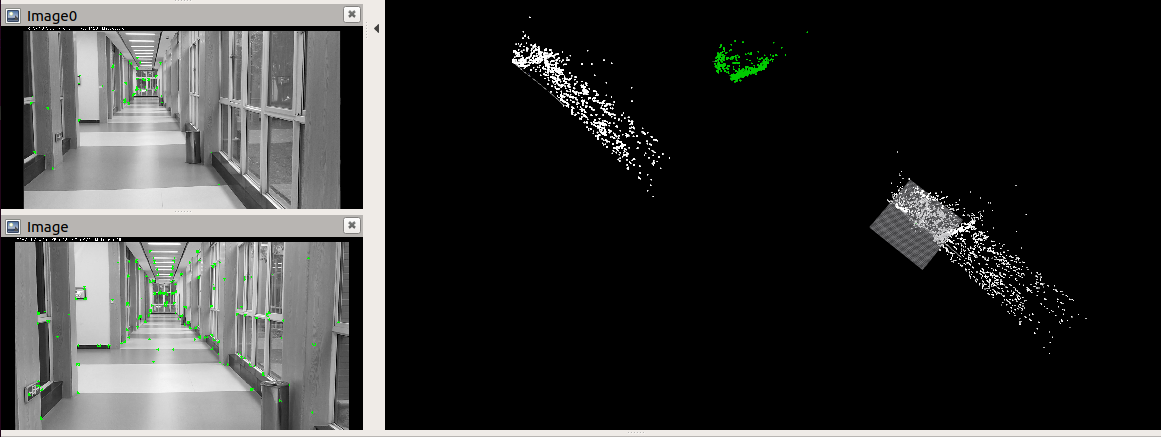
\includegraphics[width=0.9\textwidth]{ccm1.png}
	\caption{地图融合结果}
	\label{fig5-1}
\end{figure}

可以看出,基本完成了建图和地图融合的任务。

\renewcommand{\baselinestretch}{1.5}
\fontsize{12pt}{13pt}\selectfont

\chapter{总结与展望} \label{conclusion}


\section{全文总结}

SLAM技术是当今机器人以及无人系统在进入未知环境时进行运动决策和场景感知的关键技术,而可协同的SLAM方案则为集群机器人或无人系统提供了更多可能。本文主要研究了SLAM技术的原理及地图拼合的技术,基于gazebo仿真平台实现对单机和多机的视觉SLAM软件在环仿真。本文主要做的工作如下:

\begin{enumerate}
	\item 在理论上,本文剖析了ROS整体框架、话题和服务两种通信机制和gazebo仿真的概念及配置。研究了PX4 AutoPilot软件的使用,其Failsafe机制和EKF2的更改以及飞行模式,使用MAVROS进行通信的离板程序控制。了解了SLAM系统,根据相机成像原理,对其内参外参矩阵进行推导。研究了ORB-SLAM2方案中ORB特征点的定义与提取方法,分析其主要进程和主要功能函数。分析了CCM-SLAM方案中客户端与服务器的设计。
	
	\item 在仿真上,讲述了如何在gazebo平台通过launch文件配置仿真环境。实现了航路点控制和编队控制飞行的方法,开发了键盘控制的速度飞行的方法。在单机SLAM仿真中,完成了无人机在离板模式下的起飞与降落,航路点飞行;使用了新的Offboard控制程序,并且设计了从SLAM解算出的位姿到MAVROS消息类型位姿的转换方法;最终完成了基于视觉定位和速度控制的的SLAM仿真,并且获得了回环的结果。在多机SLAM仿真中,详细阐述了多机sdf文件生成模型的原理,提出了配置模型的方法,配置了具有双目和单目相机的无人机;完成了多机编队控制和航路点飞行,并且最终在一定控制策略下完成了多机的SLAM仿真。
	
	\item 在实验上,主要从真实相机、数据集、录制视频三个方面完成了实验的验证。其中使用T265相机完成了校园教学楼中的SLAM实验,获得了良好的回环结果。使用EUROC数据集,验证了双机飞行的协同SLAM方法。使用在校园场景内录制的视频,并将其转换成rosbag格式,最终获得了较为良好的地图拼合场景。
\end{enumerate}

\section{对未来工作的展望}

根据本文的分析,视觉SLAM的算法上已经有很多优秀的方案,但是在多设备利用视觉SLAM的定位和建图信息完成定位、导航等其他任务上还有很多发展余地:

\begin{enumerate}
	\item
	在理论上,针对集群的SLAM方案还比较少,其中的通信机制还比较复杂;多机地图的融合方法还存在同一的路标点无法识别导致的重复建图问题。单目ORB-SLAM2方法中,当无人机速度快时容易跟踪丢失且重定位失败的问题,这是没有IMU信息的视觉SLAM方法的问题之一;其方向是融合IMU信息,比如VINS方案和ORB-SLAM3方案,跟踪性能更好;有望开发融合UWB信息的,更加稳定的多设备协同SLAM系统,或是使用多传感器融合的SLAM方案。
	\item 
	在仿真上,倾向于使用UI界面更好,拥有更加复杂仿真能力的仿真平台;可以在Linux端完成开发,在Windows端的UE4和Airsim上完成仿真;有望在仿真中实现UWB模块和激光雷达等模块,借此实现更为复杂的仿真。
	\item 
	在实验上,本实验并没有使用真正意义上的离板模式多机SLAM,有望在研究多机的稳定飞行控制之后,使用实机进行多机编队飞行;无人机的飞行没有自主能力,有望在未来的研究中配备导航算法,使无人机能够自主地完成陌生场景的定位与建图,最终完成导航,拥有自主执行任务的能力。
	
\end{enumerate}





% reference
\renewcommand{\baselinestretch}{1.0}
\backmatter
\bibliographystyle{nwputhesis}
% \bibliographystyle{plain}  
\bibliography{reference}
% 添加目录到参考文献
\addcontentsline{toc}{chapter}{参考文献}


% acknowledgements and conclusion


\renewcommand{\baselinestretch}{1.5}
\fontsize{12pt}{13pt}\selectfont

\chapter*{致~~~~谢}
\addcontentsline{toc}{chapter}{致谢}

首先要感谢我的指导老师布树辉老师。感谢布老师在我特殊的为期接近两年的毕设进程中的指导和鼓励,从最初的C++和Opencv学习到后面的每周的组会,布老师为我指出了很多问题,同时也提出了很多醍醐灌顶的建议,感谢布老师很多次教给我的做事情先化繁为简,再由简到繁的方法;感谢布老师努力经营的Gitee平台仓库,里面涵盖了许多学习资料和实践指导,在我学习的路上提供了一条捷径;感谢布老师为我们提供的团队毕设的环境,这种每个人共同为一个目标做出贡献的感觉让我感觉自己处在一个大家庭中;布老师总告诉我实现一个目标要先实现它大概的样子,而不是纠结于一些细枝末节,在大致实现的过程中建立感性认识,之后再一点一点积累知识和方法,才能建立理性认识,这个观点让我受益匪浅。回想起来,我可能是同年级组里最早接触布老师的学生,当时老师机器学习课上30分钟学会python的方法和后来为了提前接触科研的联系,都让我明白学知识、做科研的过程中,方法很重要、有的放矢很重要,但更重要的是自律的态度、鲜明的任务规划、及时的反馈机制、对待任务的严谨,还有最重要的热爱。

还要感谢我的师兄杜万闪和李白杨,他们在我学习飞控和PX4、MAVROS相关中为我提供了莫大的帮助和环境,李白杨师兄还耐心地为我复现出现的bug并且带着我解决;感谢PI-LAB的王禹师兄,在我解决PX4的bug上提供了很大帮助。感谢我的同组同学张一竹和贾旋,他们对团队的贡献和认真的态度一直在激励着我;感谢我的室友陈泽帅为我提供了舒适的开发环境;感谢整个飞控二班在毕设的日子里愉快的氛围,Auld Lang Syne。

感谢PX4的开发团队,耐心回复我的issue;感谢stackoverflow上的程序员们,感谢ROS论坛、古月居、ORB-SLAM2和CCM-SLAM的作者、XTDrone平台。

最后要感谢我的父母对我一如既往的关心。
感谢我的女朋友,遇到你是我大学生活里最幸运的事。是你让我以后的生活有了明确的目标和期待,更重要的是有了和我一起期待未来的人。写到致谢时才回过头看了看这四年的自己,才发现大学四年即将结束,希望自己能做一个带着回忆又勇敢向前追逐的人,江头潮平,但斯人会归。


\chapter*{毕业设计小结}
\addcontentsline{toc}{chapter}{毕业设计小结}

本次毕业设计与飞控专业的相关度可能不高,只是使用了飞控的硬件和软件,也不要求我掌握具体的动力学模型和控制律。但本次毕设注重于崭新的机器人方向和计算机视觉技术(主要是视觉SLAM),注重于对编程能力的提升。虽然以XTDrone的仿真平台为样本,但是每一个launch文件和更改的SLAM代码都出自自己之手,在不断的尝试和分析过程中开始对ROS环境下的仿真有了更加深层的了解。

本次毕设的难点集中在仿真环境的底层机制和SLAM方案上,尤以SLAM方案为主。无论是ORB-SLAM2还是CCM-SLAM,都是十分优秀的开源方案。但面对一套完整的现代的SLAM方案时,一开始会无从下手,面对数量众多的源代码和头文件,以及源代码中众多类的众多函数,会难以分析该程序的数据流。但是经历这次毕设,让我逐渐掌握了针对这种大型方案快速学习的方法,这一点对日后遇到类似的方案并进行二次开发时会有很大帮助。

经历了这次毕设,我对SLAM技术有了更深的了解,对Linux操作系统也比较熟悉,对ROS的相关用法有了初步认识,提高了自己对PX4的debug能力。





\end{document}

